\section{PIV: studio della scia di corpi tozzi}
Lo scopo della presente attività è il calcolo dei campi di velocità nella scia di corpi tozzi mediante la tecnica Time Resolved Particle Image Velocimetry (TR-PIV) utilizzando uno smartphone ed una lama di luce di bassa potenza.

\subsection{Descrizione dell'esperimento}
La Particle Image Velocimetry (PIV) è una tecnica ottica non invasiva che consente di valutare campi istantanei di velocità caratterizzati da un elevato numero di vettori velocità.\\\\
Nella sua continua evoluzione, la metodologia PIV ha dato luogo a forme sempre più sofisticate e complete ai fini della determinazione del campo del vettore velocità istantaneo:
\begin{equation*}
    \vec V (t, x, y)
\end{equation*}
La valutazione della velocità in ogni punto del campo discende direttamente dalla definizione di velocità:
\begin{equation*}
    V = \frac{\Delta s}{\Delta t}
\end{equation*}
La tecnica richiede l'immissione di particelle nel campo che consentono la valutazione della velocità della corrente attraverso il calcolo dello spostamento $\Delta s$. L'intervallo di tempo $\Delta t$ è invece impostato sul sistema dall'operatore.\\\\
La tecnica PIV è caratterizzata da una elevata risoluzione spaziale dovuta alle caratteristiche della telecamera utilizzata. Infatti, in relazione alle dimensioni del campo fisico ripreso il numero di vettori calcolati per unità di superficie dell'immagine ripresa risulta essere molto elevato e tale da rendere la misura tendente al puntiforme. Questo consente di descrivere il campo di moto dettagliatamente nello spazio evidenziando accuratamente le regioni caratterizzate da elevati gradienti di velocità.\\\\
La configurazione Time Resolved Particle Image Velocimetry (TR-PIV) associa l'elevata risoluzione spaziale ad una buona risoluzione temporale che consente di campionare le immagini fino a diverse migliaia di fotogrammi al secondo. Rispetto alla risposta in frequenza della tecnica anemometrica a filo caldo e a quella dell'anemometria LDA quella della tecnica PIV è molto più bassa.\\\\
La sorgente laser emette un raggio luminoso, coerente e monocromatico, che viene fatto espandere attraverso un sistema di lenti generando un piano di luce di spessore molto piccolo.\\\\
La tecnica prevede l'inseminazione della corrente da esaminare mediante particelle iniettate a monte o direttamente nel campo di moto attraverso un sistema di inseminazione. Le particelle, attraversando il piano di luce, sono illuminate e riflettono rendendosi visibili alla telecamera, che ne riprende la loro posizione. L'inseminazione deve essere caratterizzata da una densità di particelle elevata, come regola empirica ogni "area di interrogazione" deve contenere come ordine di grandezza dieci particelle.\\\\
La telecamera deve essere posizionata perpendicolarmente al piano illuminato e deve acquisire le immagini PIV, sulle quali sono riportate le tracce delle particelle illuminate. Le immagini sono costituite da un numero di righe di pixel $M$ e da un numero di colonne di pixel $N$, che individuano il numero totale di pixel. Si definisce quindi risoluzione il prodotto tra $N$ e $M$.\\\\
Da un punto di vista matematico, l'immagine è definita da una funzione che descrive l'intensità del livello di grigio nel piano $x$-$y$ dell'immagine ripresa:
\begin{equation*}
    I = f(x,y)
\end{equation*}
Il livello di grigio è indicato in modo discreto, ad ogni pixel viene quindi assegnato un valore numerico compreso tra 0 e $2^n$, dove $n$ è il numero di bit.\\\\
Ogni immagine PIV viene suddivisa in aree di interrogazione $A_N$ tipicamente quadrate e di dimensioni uguali tra loro. In ogni area di interrogazione ricade un certo numero di particelle, per ogni area viene quindi calcolato lo spostamento delle particelle contenute. L'area di interrogazione deve essere sufficientemente piccola in modo tale da poter ritenere il flusso uniforme, non deve essere troppo grande in quanto si rischia di perdere la descrizione dettagliata del campo. Più l'area è grande e meno verificata sarà la condizione di flusso uniforme.\\\\
Contemporaneamente, l'area di interrogazione deve contenerre un numero minimo di particelle (dell'ordine di dieci) affinché sia possibile valutare uno spostamento statistico affidabile attraverso gli algoritmi di calcolo.\\\\
L'analisi delle immagini per la determinazione degli spostamenti delle particelle può essere effettuata in due diversi domini:
\begin{itemize}
    \item Nel dominio dello spazio mediante la valutazione della funzione di autocorrelazione per immagini multi-esposte (poco utilizzata) e della funzione di cross-correlazione nel caso di immagini singolarmente esposte, questa nel continuo è definita come:
    \begin{equation*}
        R_{j,j+1}(r_1,r_2) = \iint_{A_N} F_j(x,y)F_{j+1}(x+r_1,y+r_2)dxdy
    \end{equation*}
    Nel discreto, la funzione di cross-correlazione si calcola come:
    \begin{equation*}
        R_{j,j+1}(r_1,r_2) = \sum_{h=1}^{\Delta h}\sum_{k=1}^{\Delta k} F_j(h,k) F_{j+1}(h+r_1, k+r_2)\Delta h \Delta k
    \end{equation*}
    \item Nel dominio delle frequenze mediante la valutazione della Fast Fourier Transform (FFT) di due immagini successive. È il procedimento operativo che si segue perché risulta del tutto equivalente al procedimento di analisi mediante cross-correlazione ma risulta essere molto più veloce.
\end{itemize}

\noindent La FFT è un algoritmo per calcolare la Trasformata di Fourier Discreta (DFT) in modo efficiente. La DFT di una sequenza $f(x)$ è definita come:
\begin{equation*}
    \mathcal F(k) = \sum_{n=0}^{N-1} f(n) e^{-i 2 \pi k n / N}
\end{equation*}
La cross-correlazione può essere calcolata utilizzando la FFT tramite il teorema di convoluzione:
\begin{equation*}
C(x, y) = \mathcal{F}^{-1} \{ \mathcal{F}[A(x, y)] \cdot \mathcal{F}[B(x, y)]^* \}
\end{equation*}
dove $\mathcal{F}$ denota la trasformata di Fourier e $\mathcal{F}^{-1}$ l'antitrasformata, mentre con l'apice "$^*$" si denota il complesso coniugato.\\\\
Mediante questi algoritmi numerici, la cross-correlazione di ciascuna area di interrogazione tra due immagini successive permette di determinare lo spostamento delle particelle e quindi il campo di velocità del fluido.

\subsection{Catena di misura}
L'esperimento viene condotto in un canale idrodinamico a pelo libero, il cui flusso è messo in moto da un'elica spingente azionata da un motore brushless. I corpi analizzati (cilindro o placca piana) sono posizionati nella camera di prova del canale in condizione di bassi regimi di numero di Reynolds. La bassa velocità del flusso permette di utilizzare la telecamera di uno smartphone.
\begin{figure}[H]
    \centering
    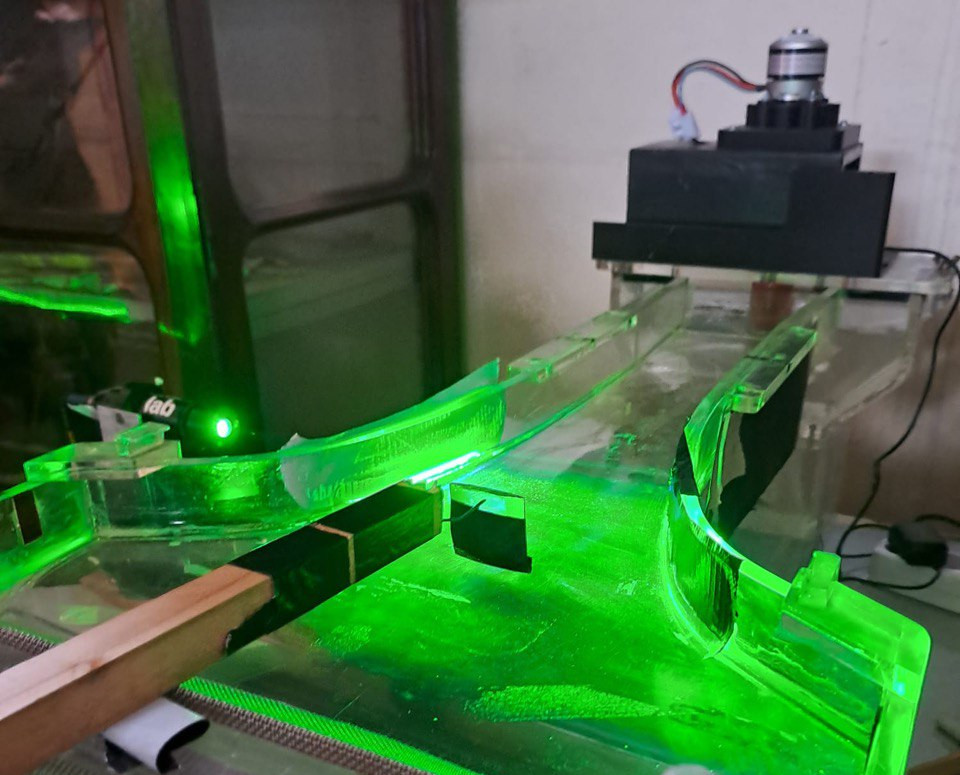
\includegraphics[height=.46\textwidth]{images/11/piv1.jpg}
    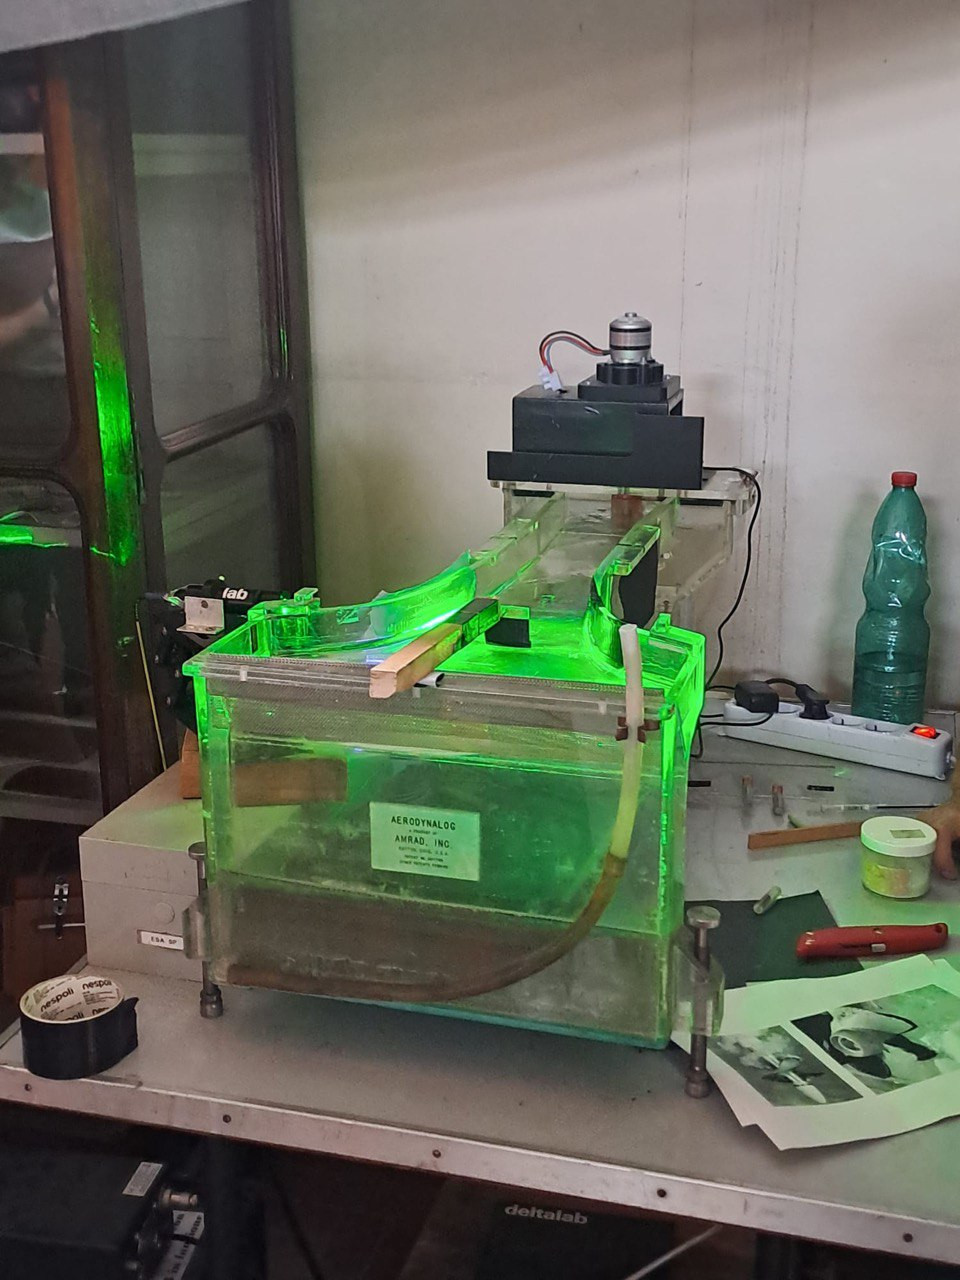
\includegraphics[height=.46\textwidth]{images/11/piv2.jpg}
    \caption{Canale idrodinamico}
\end{figure}

\noindent Nel caso del cilindro, il flusso che si sviluppa non risulta essere quello canonico 2D per via della sua dimensione finita che appoggia sulla parete inferiore della camera di prova. Inoltre, il piano di misura è a un diametro di distanza dal fondo, dove si sviluppa il vortice a ferro di cavallo (horseshoe vortex) e sono presenti effetti tridimensionali dovuti all'induzione del vortice. Per questi motivi i casi da studiare differiscono dai flussi canonici bidimensionali, pertanto, l'andamento Reynolds-Strouhal potrebbe discostarsi da quello studiato per il cilindro 2D utilizzando l'anemometria a filo caldo.\\\\
I corpi analizzati sono un cilindro (diametro $d=10$ mm) ed una placca piana rettangolare (lunghezza $L=24$ mm).
\begin{figure}[H]
    \centering
    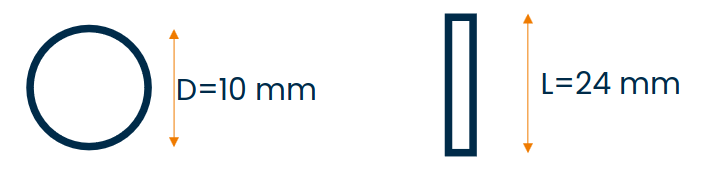
\includegraphics[width=.5\textwidth]{images/11/rapprcorpi.png}
    \caption{Sezione dei corpi tozzi in esame}
\end{figure}

\noindent Per le misure si utilizza un sistema PIV "low cost", costituito dalla telecamera di uno smartphone la cui risoluzione è di 1920$\times$1080 pixel e frequenza di acquisizione delle immagini $f_{samp}$ pari a 60 fotogrammi al secondo, che corrisponde ad un intervallo temporale $\Delta t = 16.7$ ms.
\begin{figure}[H]
    \centering
    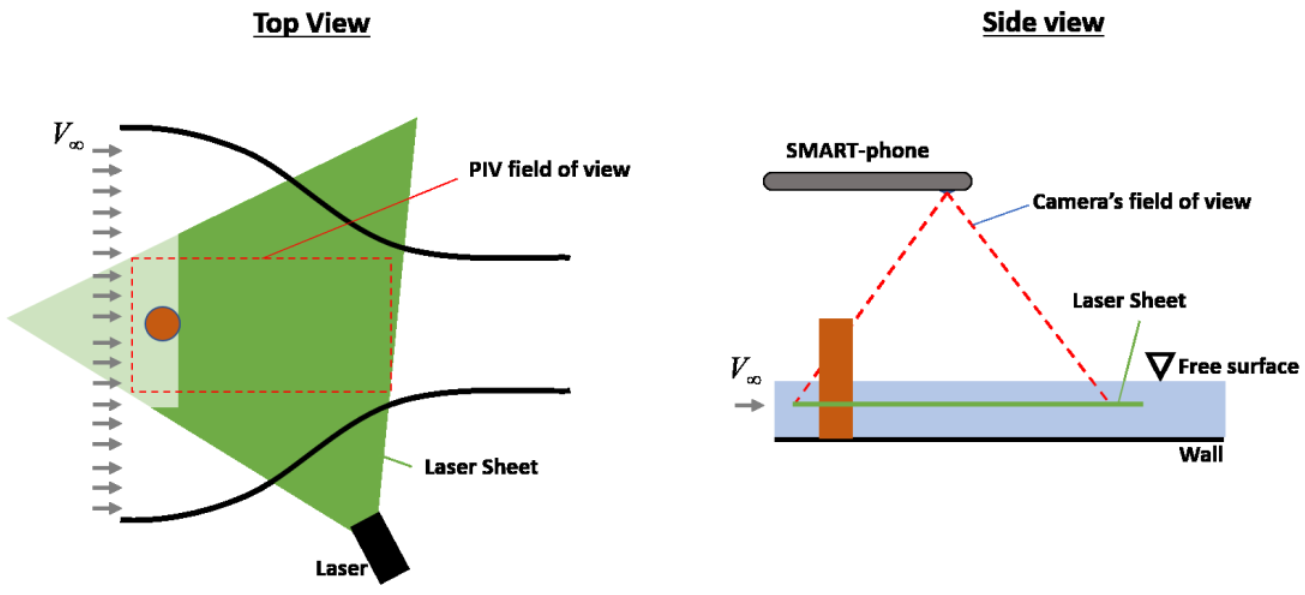
\includegraphics[width=.8\textwidth]{images/11/rapprcatena.png}
    \caption{Rappresentazione del setup sperimentale}
\end{figure}

\noindent Le particelle impiegate sono costituite da carbonato di silice ($\rho_p$=1.1 g/cm$^3$, $d_p$=2$\mu$m).\\\\
La sorgente laser ha una potenza di 30 mW e genera un fascio di luce continuo con lunghezza d'onda di 532 nm (colore verde). Una lente cilindrica, montata direttamente nella testa della sorgente laser, diverge il fascio laser lungo una sola direzione creando la lama di luce (laser sheet).\\\\
In questa configurazione viene a mancare il sincronismo tra telecamera e lama di luce, poiché l'emissione della sorgente laser è continua.
\begin{figure}[H]
    \centering
    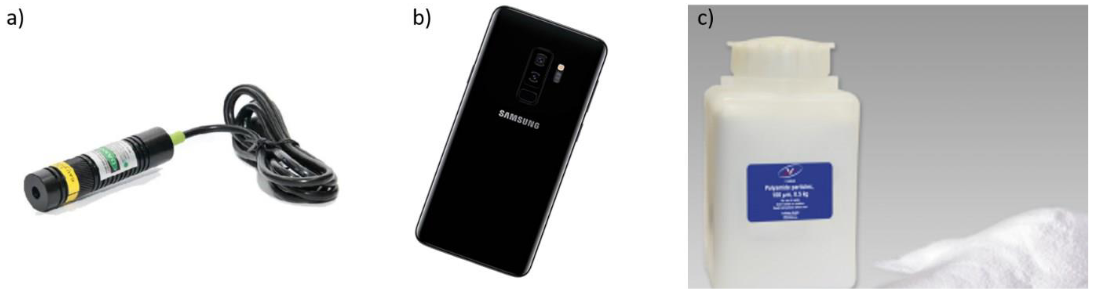
\includegraphics[width=.7\textwidth]{images/11/catenastrumenti.png}
    \caption{Sorgente laser, smartphone, particelle di poliammide}
\end{figure}

\noindent Le immagini ottenute hanno un fattore di scala $Sc$ [mm/pixel] da determinare, che deve essere usato per la calibrazione geometrica, cioè per trasformare lo spostamento misurato in pixel sulle immagini PIV acquisite in millimetri di spostamento al vero.

\subsection{Procedura sperimentale}
Per acquisire le immagini PIV, prima si mette in moto il fluido, già inseminato con le particelle di carbonato di silice, nel canale idrodinamico mediante il motore brushless che aziona un'elica spingente, facendo attenzione a non incorrere in fenomeni di cavitazione.\\\\
Successivamente si accende la sorgente laser, da cui si genera la lama di luce che attraversa il condotto nella camera di prova illuminando le particelle.\\\\
Poi si posiziona il corpo (cilindro o placca piana) a monte della camera di prova e mediante uno smartphone (che deve essere opportunamente posizionato e stabile) si registra un video di circa 10 secondi ad una risoluzione di 1920$\times$1080 a 60 fotogrammi al secondo.\\\\
Per analizzare le immagini si utilizza PIVlab, un tool box di Matlab che offre un'interfaccia grafica intuitiva per calcolare la distribuzione della velocità nei vari fotogrammi.
\begin{figure}[H]
    \centering
    
\includegraphics[width=.4\textwidth]{images/11/pivlabui.png}
    \caption{Interfaccia di avvio di PIVlab}
\end{figure}

\noindent PIVlab permette di importare le immagini, pre-processarle per migliorare il contrasto tra particelle e sfondo (se necessario) e applicare la calibrazione geometrica.
\begin{figure}[H]
    \centering
    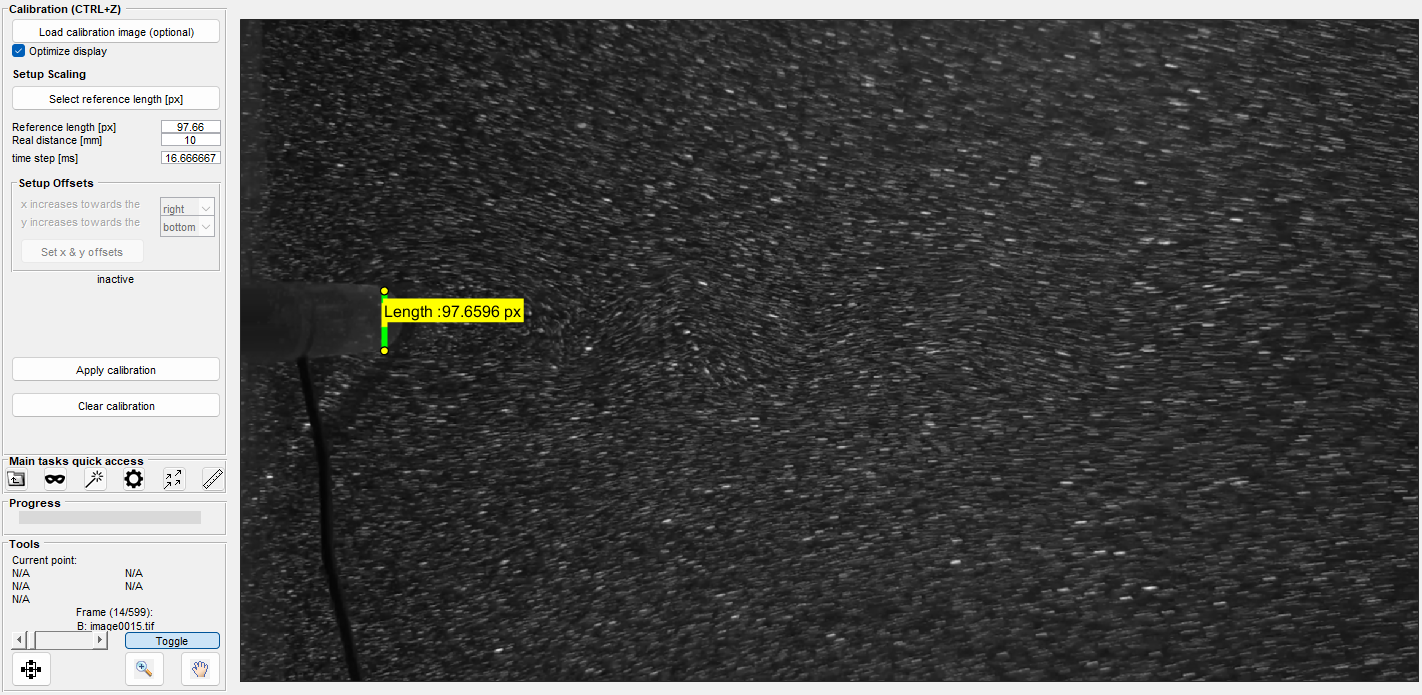
\includegraphics[width=\textwidth]{images/11/pivlabcg.png}
    \caption{Calibrazione geometrica in PIVlab (cilindro 2022)}
\end{figure}

\noindent Applicando la calibrazione geometrica si ricava lo scaling factor:
\begin{equation*}
    Sc = \frac{10\text{ mm}}{97.6596\text{ px}} = 0.1024\ \frac{\text{mm}}{\text{px}}
\end{equation*}
Poiché la frequenza di acquisizione dei fotogrammi è pari a 60 Hz ($\Delta t = 16.67$ ms), si può stimare il valore di velocità equivalente allo spostamento di un pixel in due fotogrammi successivi:
\begin{equation*}
    1\   \frac{\text{px}}{\text{frame}} = \frac{0.1024 \text{ mm}}{16.67 \text{ ms}} = 0.0061\ \frac{\text{m}}{\text{s}}
\end{equation*}
Ovviamente il valore dello scaling factor $Sc$ varia a seconda del caso in esame.\\\\
Il toolbox PIVlab comprende gli algoritmi numerici della PIV con cui si può valutare il generico campo di velocità istantaneo per ogni coppia di immagini PIV acquisite. I campi di velocità calcolati da PIVlab vengono infine esportati come file \texttt{.mat}, da fornire in input a Matlab per effettuare l'analisi dati.

\newpage
\subsection{Analisi dati}
L'analisi dati per la presente attività è condotta con l'ausilio di alcuni codici in Matlab, riportati in appendice \ref{b11}.\\\\
I file \texttt{.mat} esportati da PIVlab contengono i campi di velocità per ciascun fotogramma dei video analizzati. Utilizzando un codice Matlab, è possibile generare delle animazioni che mostrano il campo di velocità, con una scala di colori per rappresentare l'intensità e delle frecce per indicare la direzione del flusso.\\\\
\begin{figure}[H]
    \centering
    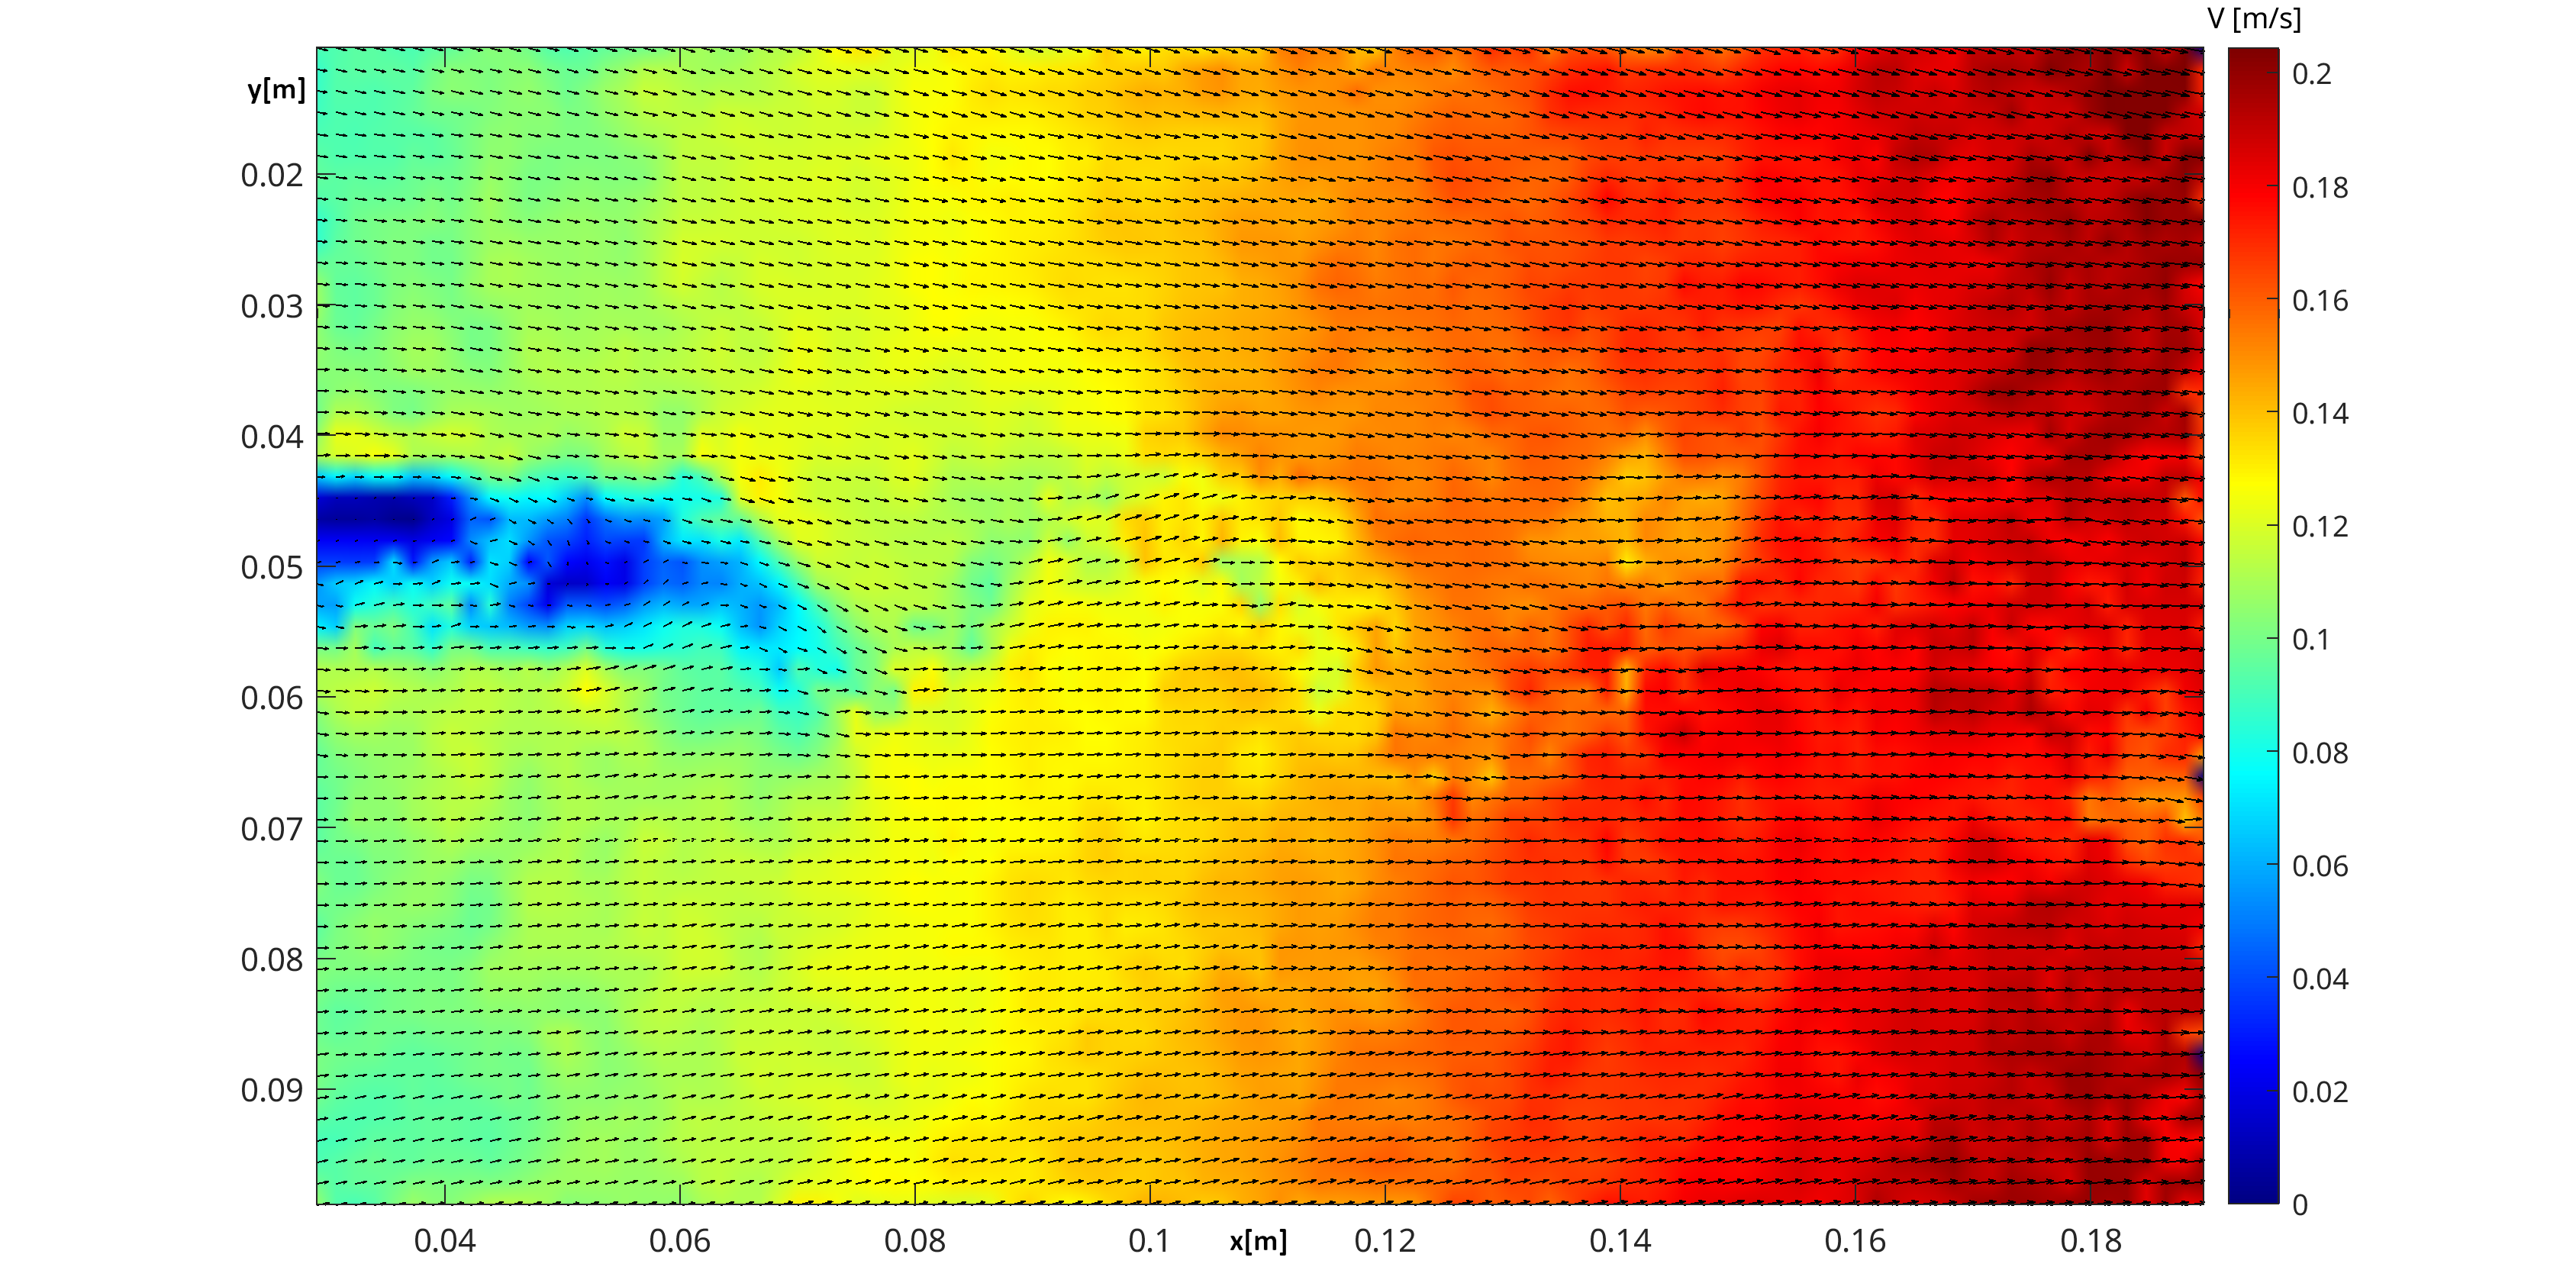
\includegraphics[height=.52\textwidth]{images/11/f300_22b.png}
    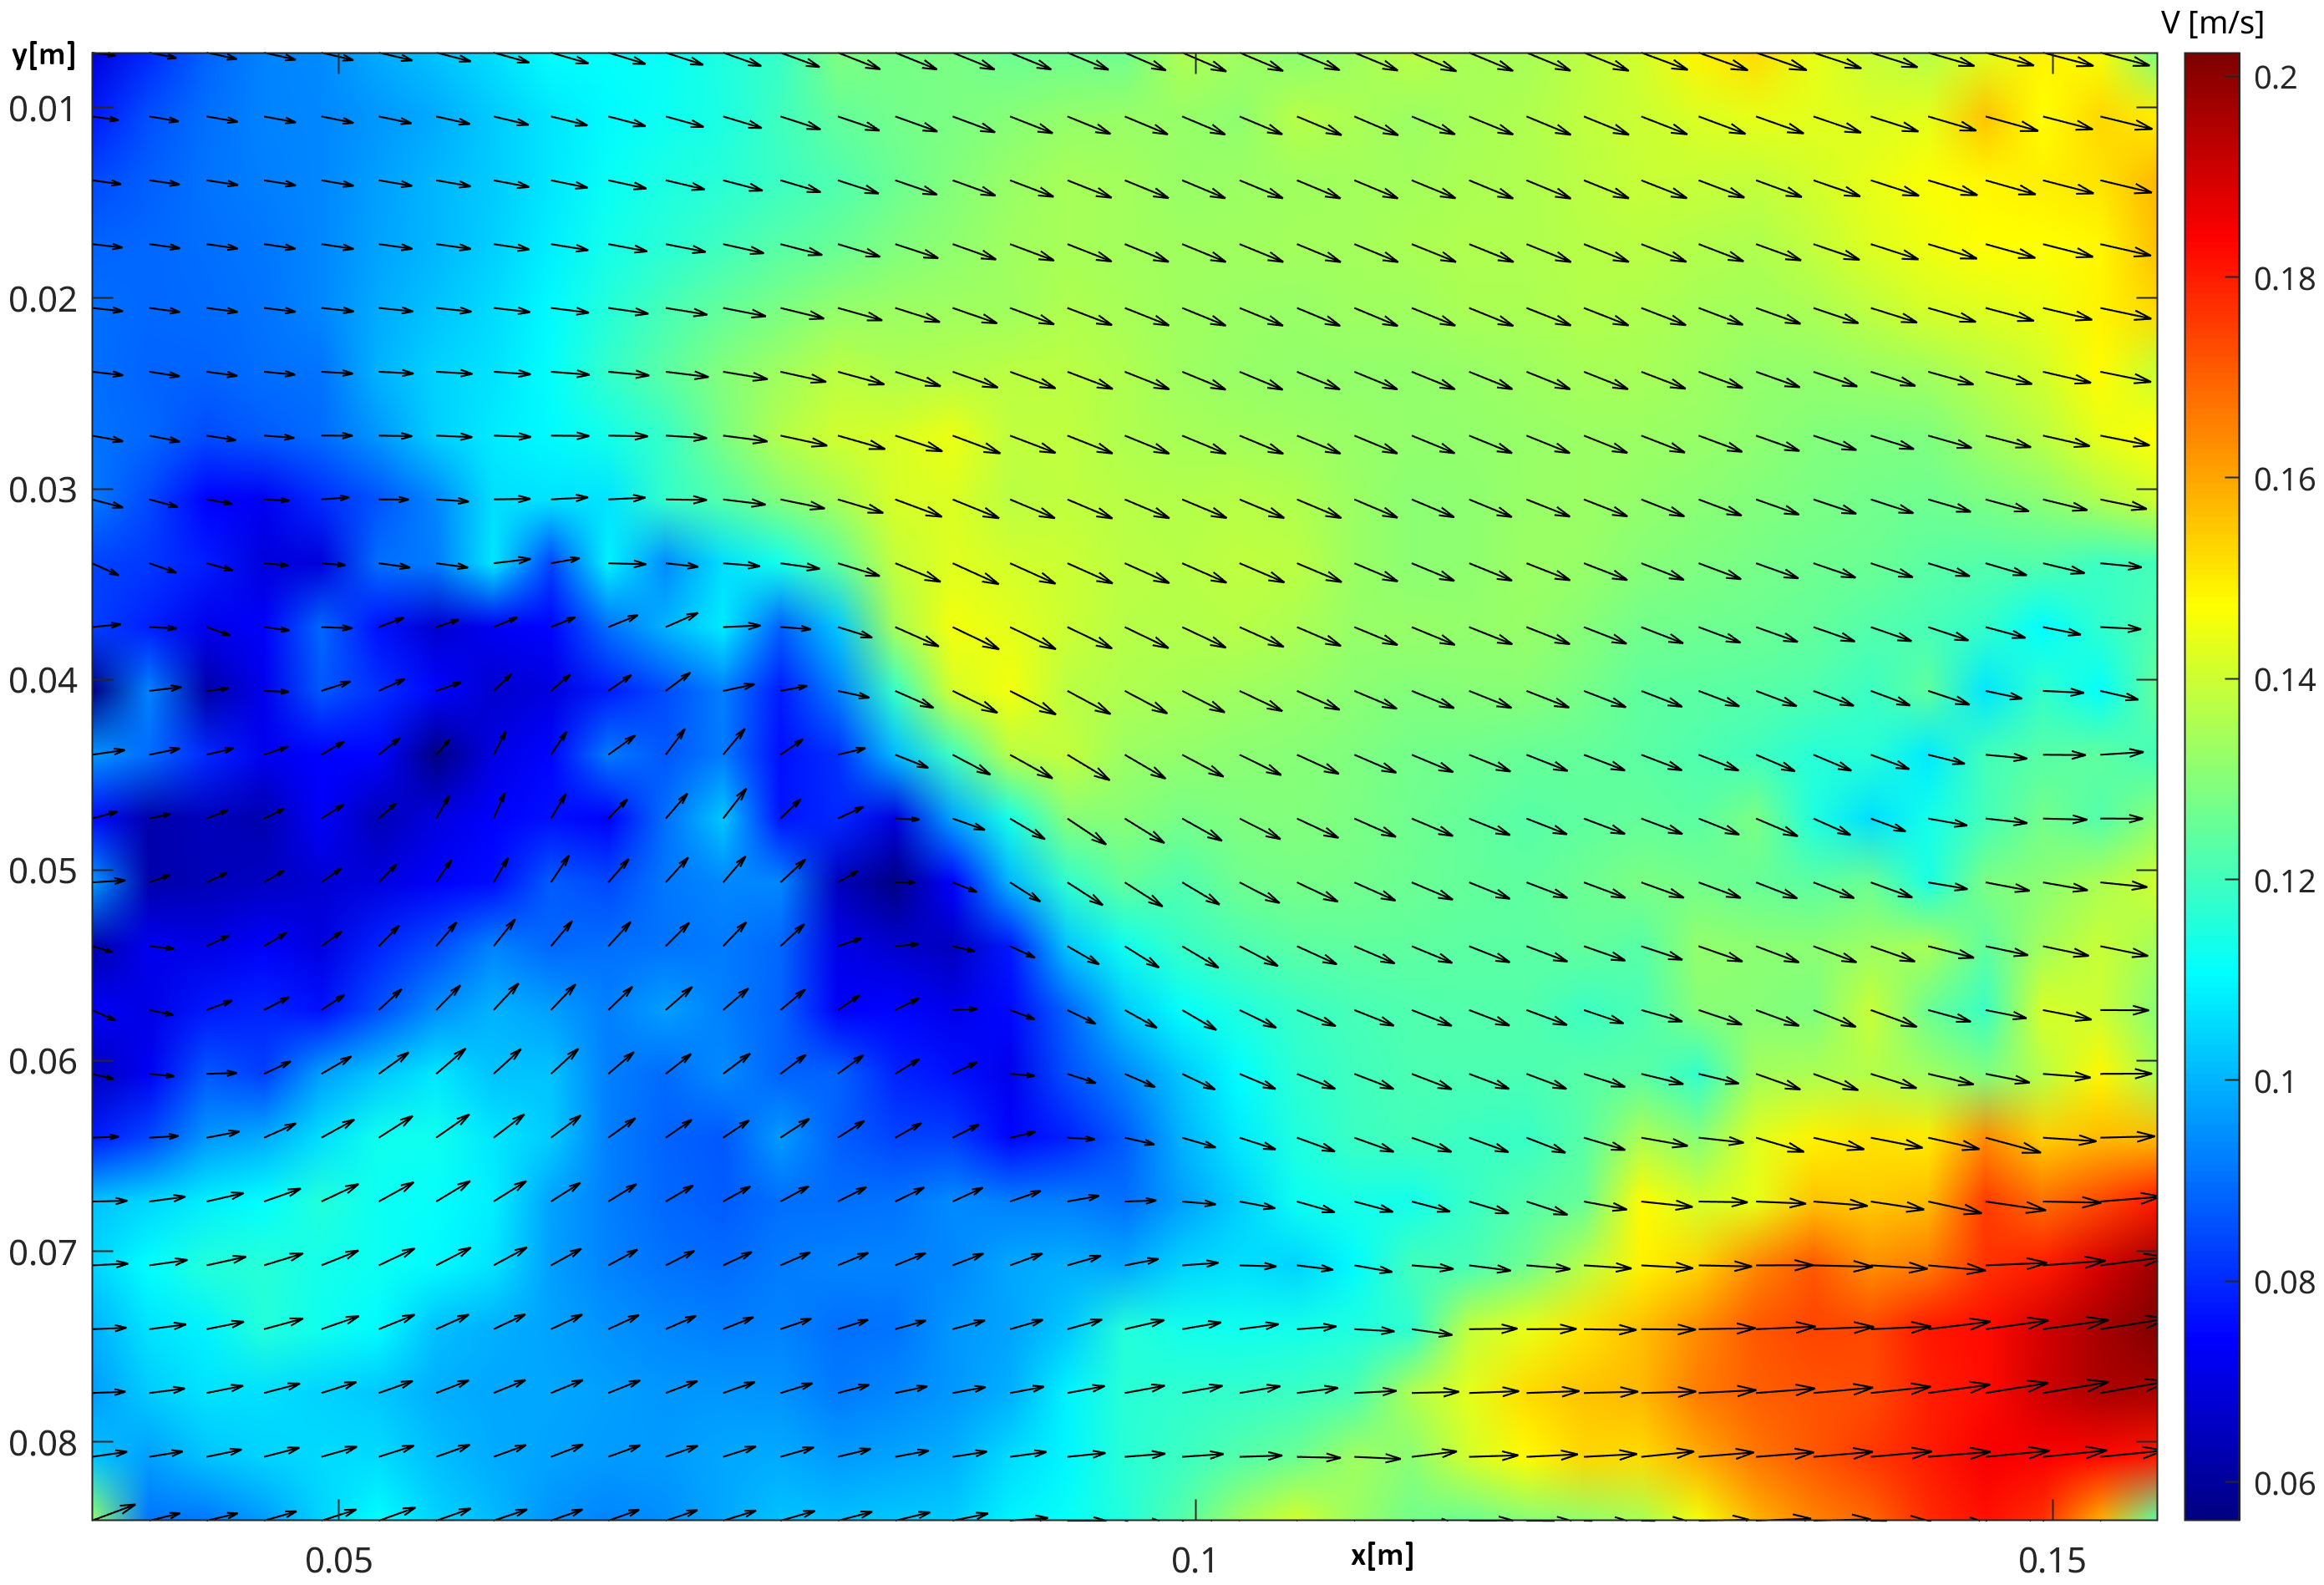
\includegraphics[height=.5\textwidth]{images/11/f300_220.png}
    \caption{Campo istantaneo di velocità (cilindro e placca 2022)}
\end{figure}

\noindent Il campo di velocità non è calcolato in tutti i pixel del video, bensì solo in una regione di interesse (ROI). Si può pensare di sovrapporre il campo di velocità ottenuto da PIVlab ai fotogrammi dei video utilizzati:
\begin{figure}[H]
    \centering
    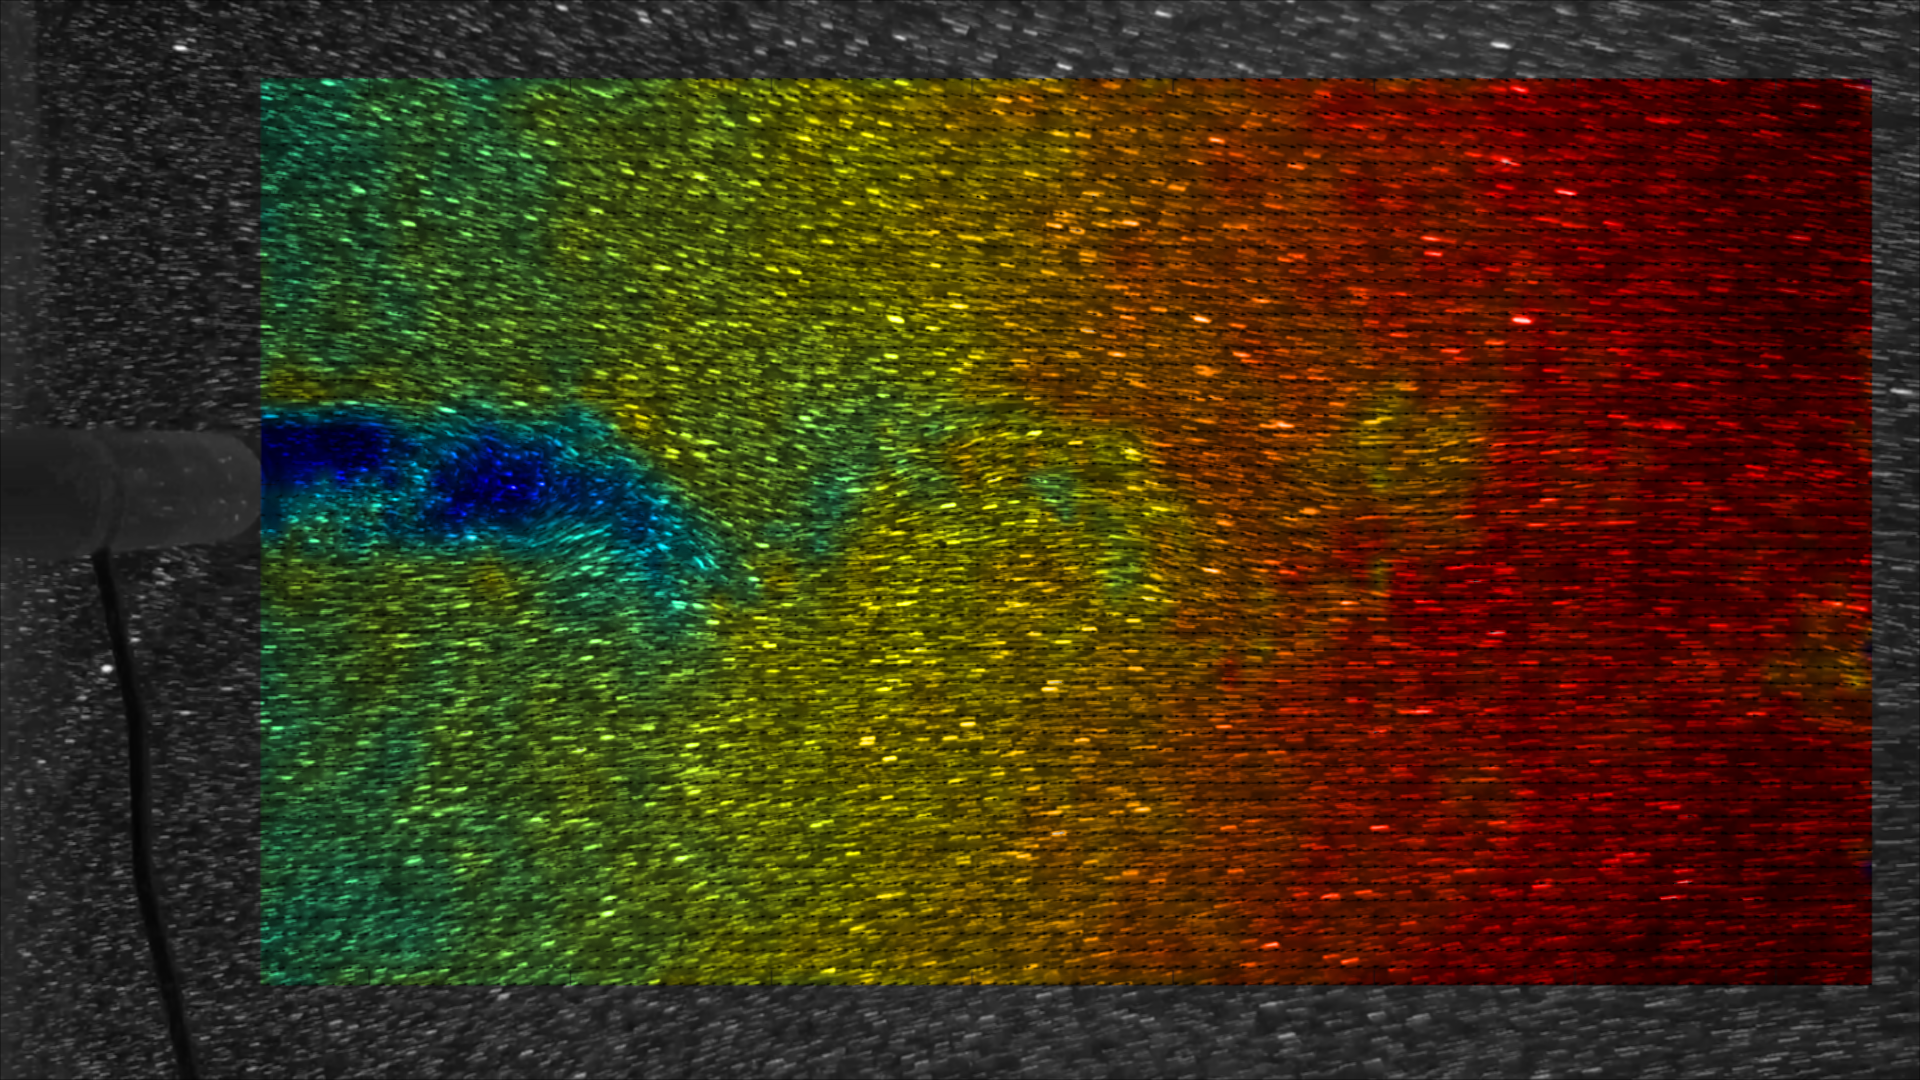
\includegraphics[width=\textwidth]{images/11/overlapped.png}
    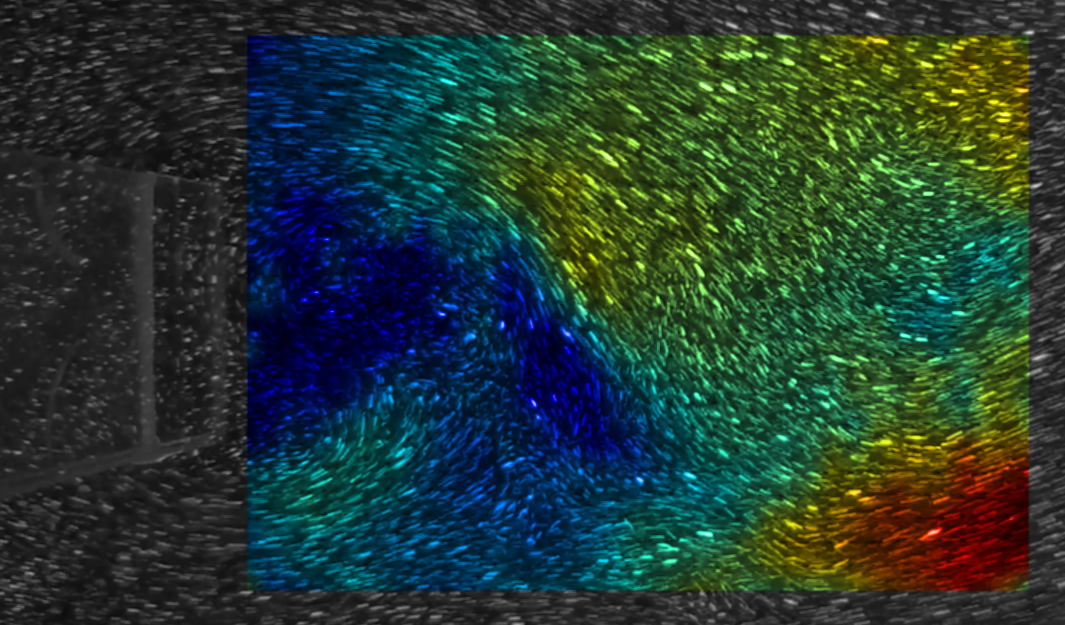
\includegraphics[width=\textwidth]{images/11/overlap_220.png}
    \caption{Campi istantanei di velocità sovrapposti ai fotogrammi dei video}
\end{figure}

\noindent Si osserva come il flusso aumenta di velocità, ciò è dovuto alla geometria convergente del canale idrodinamico. Si osserva inoltre molto chiaramente lo sfilamento vorticoso.\\\\
Mediando i campi di velocità di tutti i fotogrammi, si ottiene il seguente diagramma:
\begin{figure}[H]
    \centering
    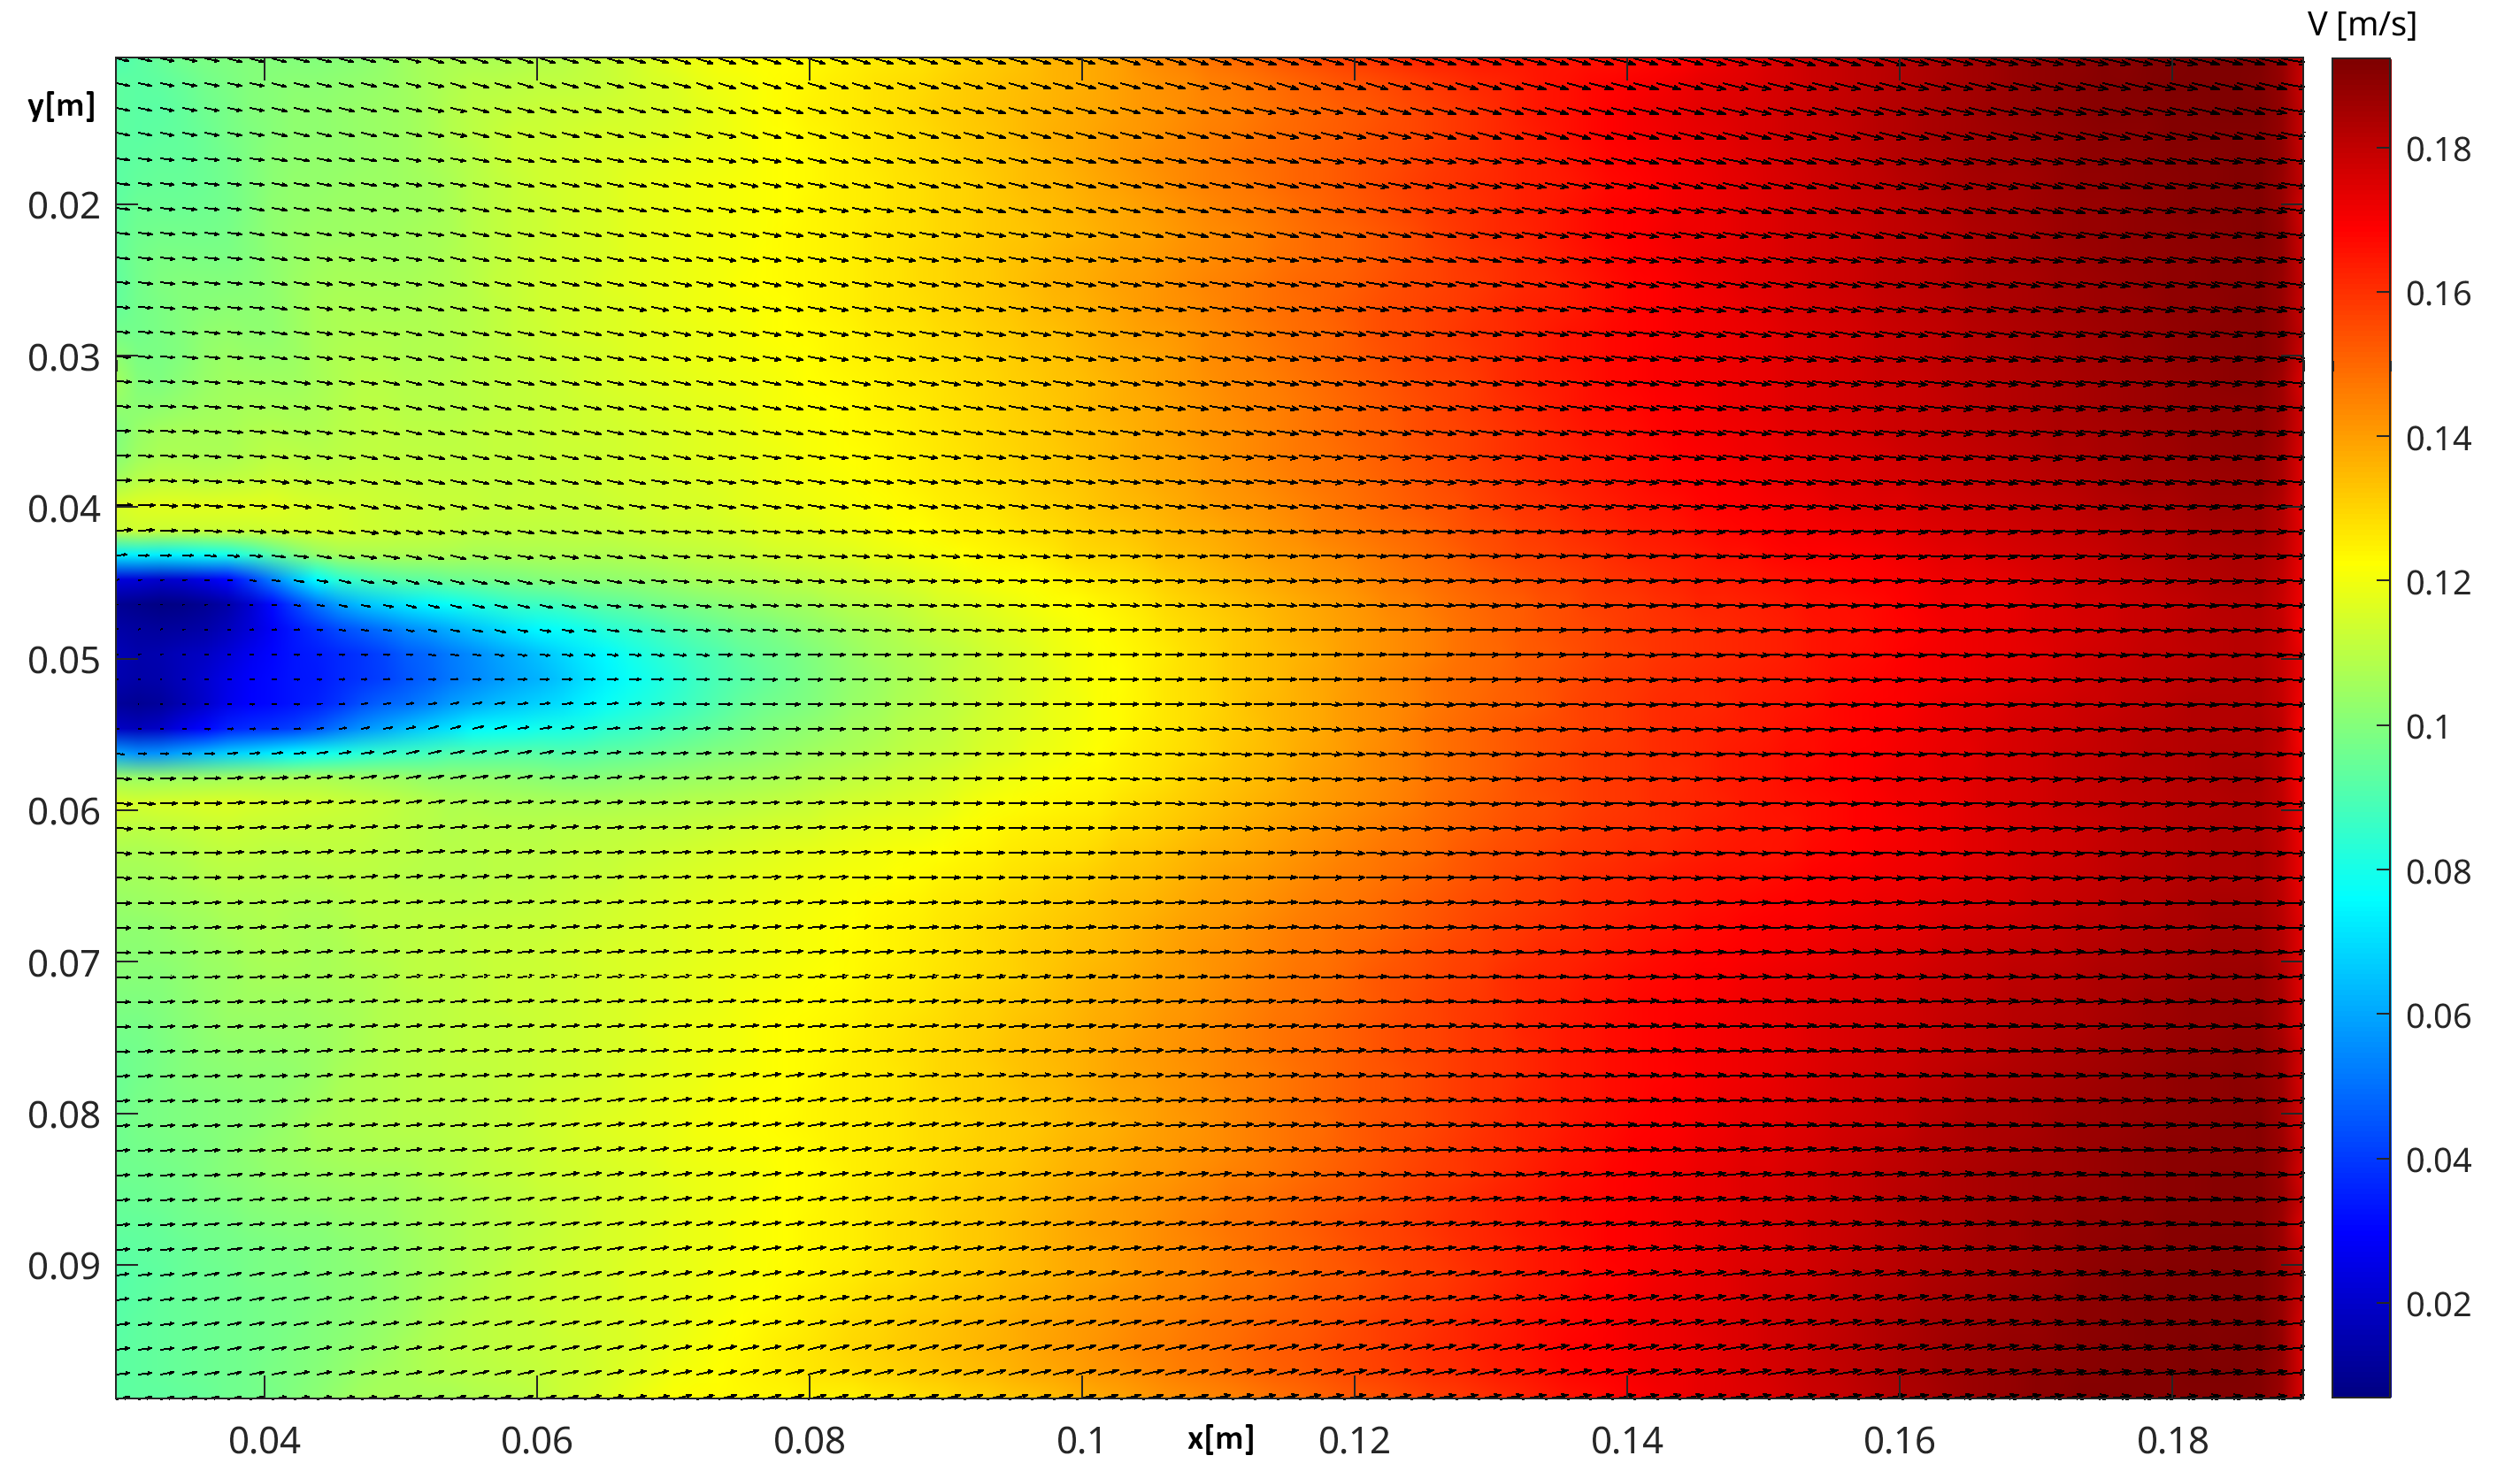
\includegraphics[width=.92\textwidth]{images/11/mean.png}
    \caption{Campo medio di velocità (cilindro 2022)}
\end{figure}

\noindent Si può pensare di mediare solo le componenti longitudinali $u$ e trasversali $v$ al condotto:
\begin{figure}[H]
    \centering
    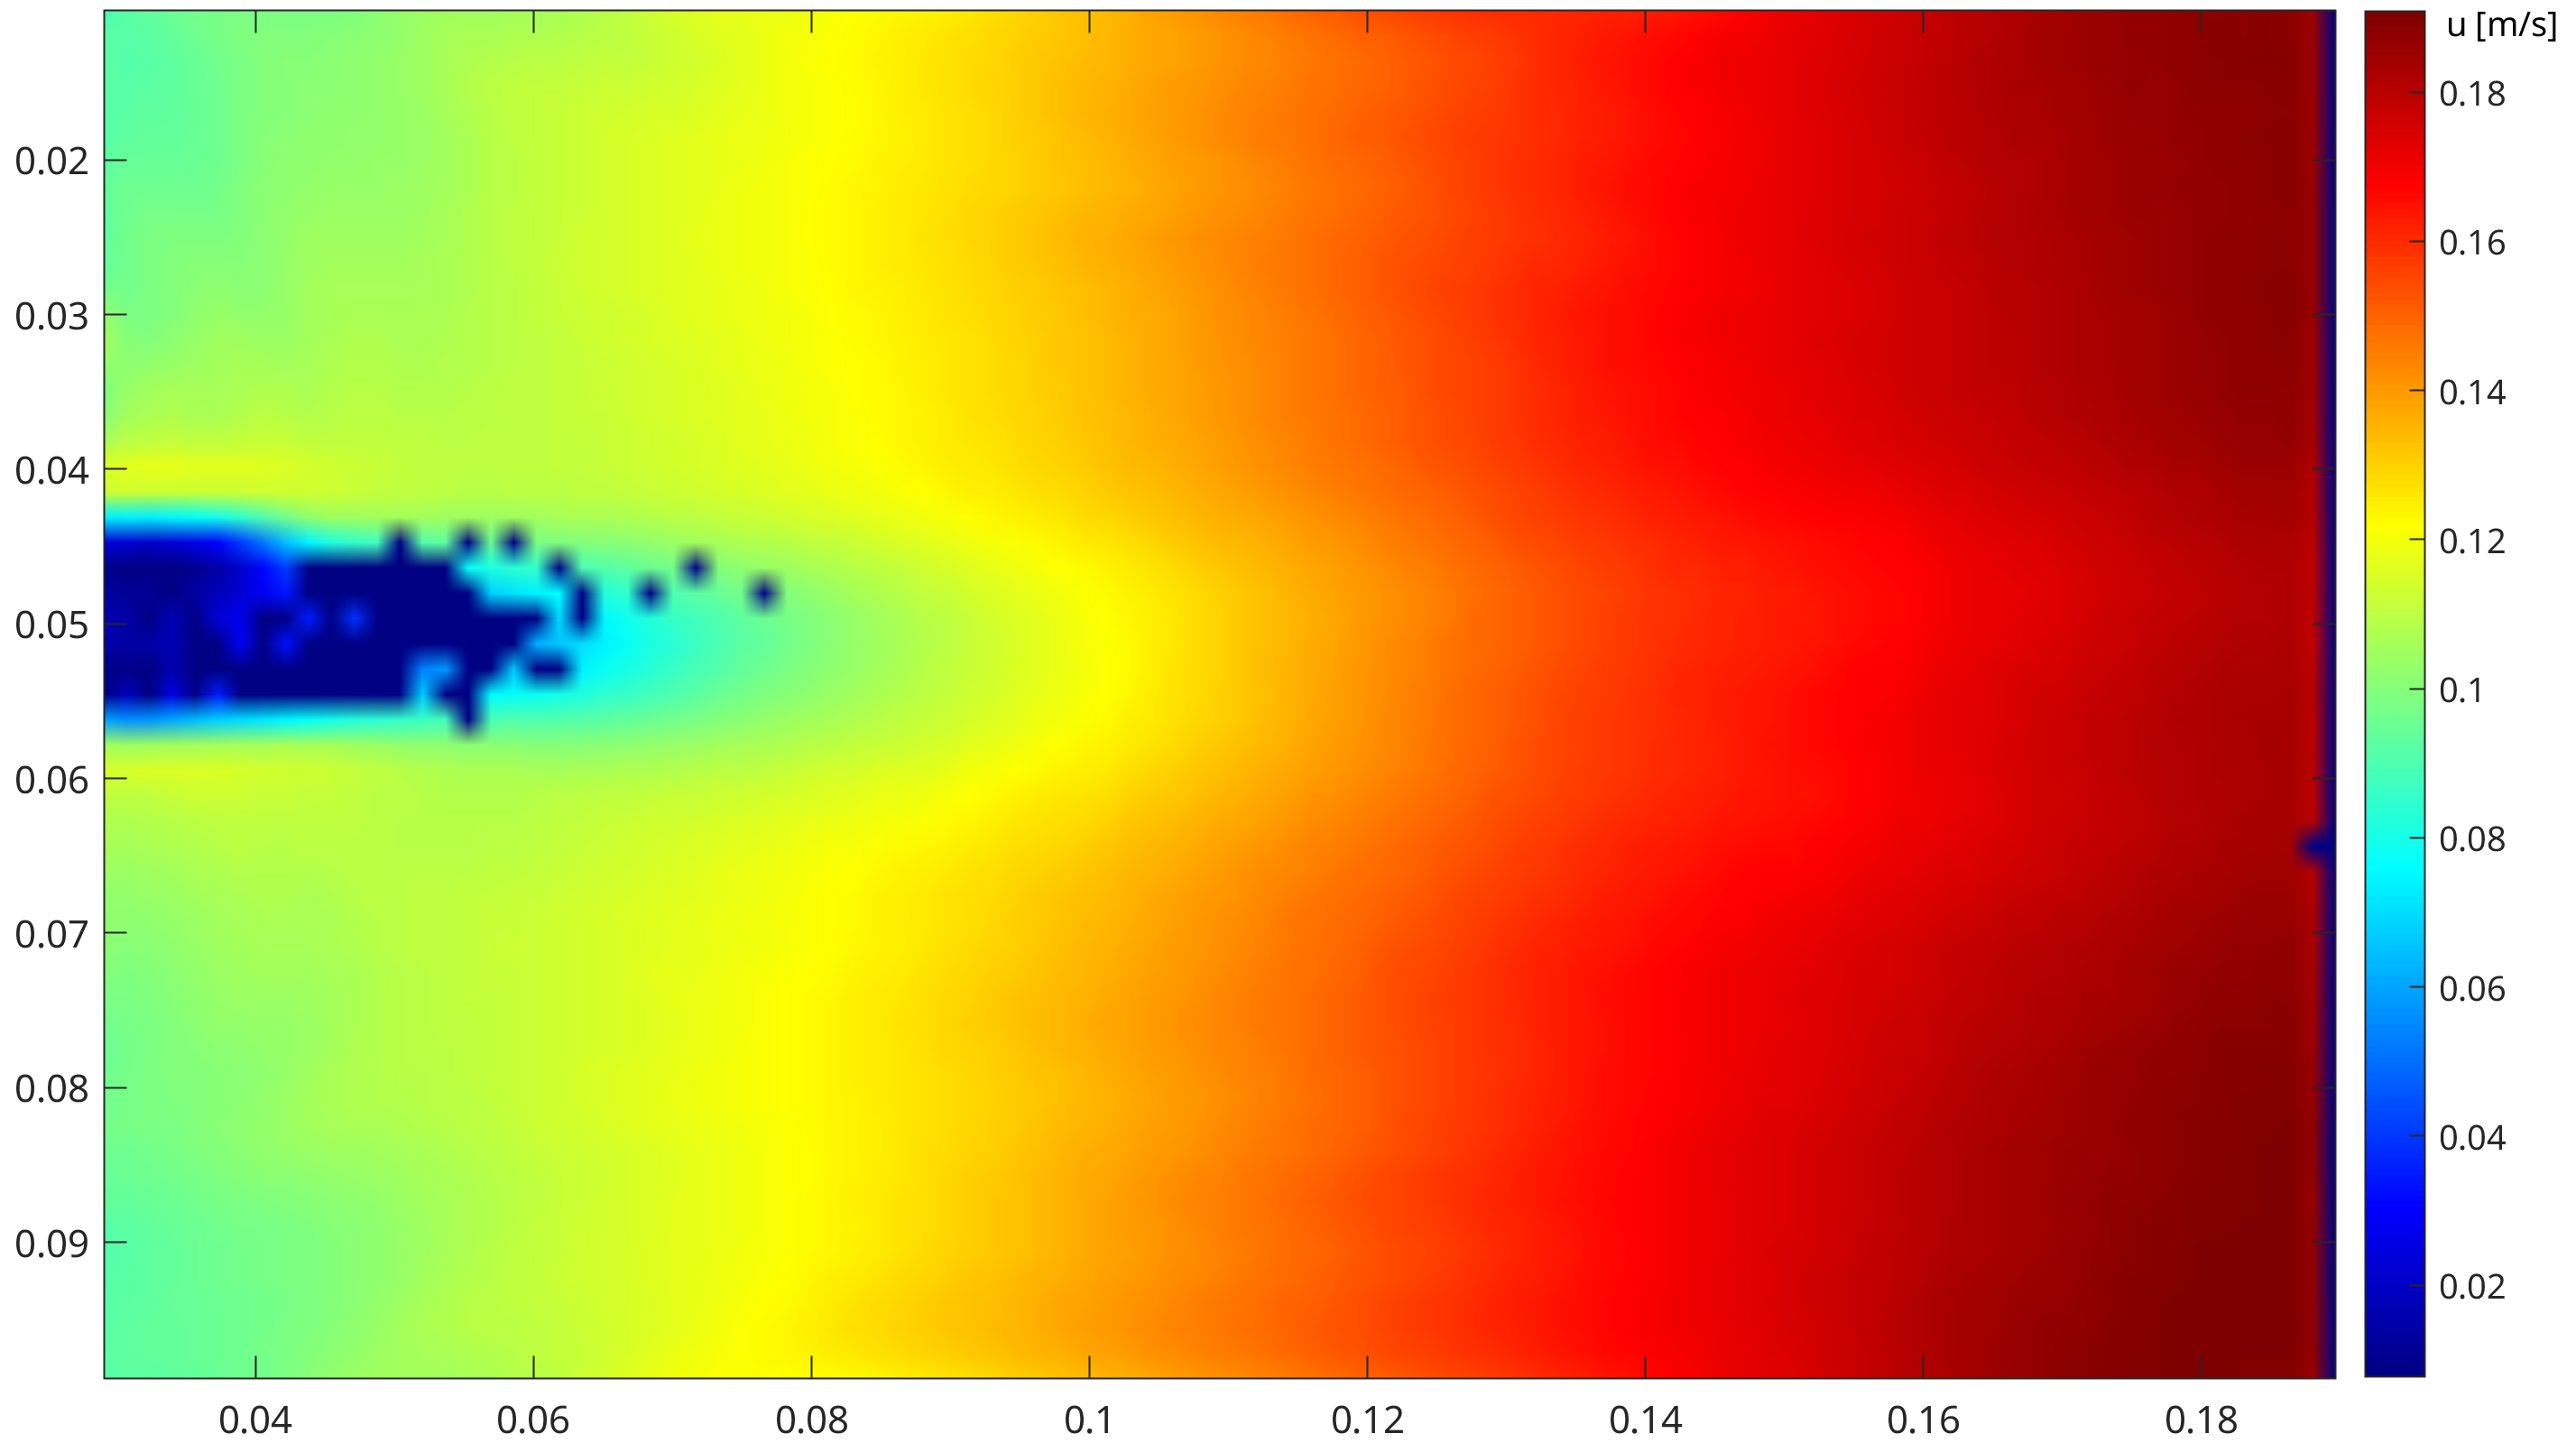
\includegraphics[width=.92\textwidth]{images/11/Umean.png}
    \caption{Componente longitudinale della velocità media $u$ (cilindro 2022)}
\end{figure}

\begin{figure}[H]
    \centering
    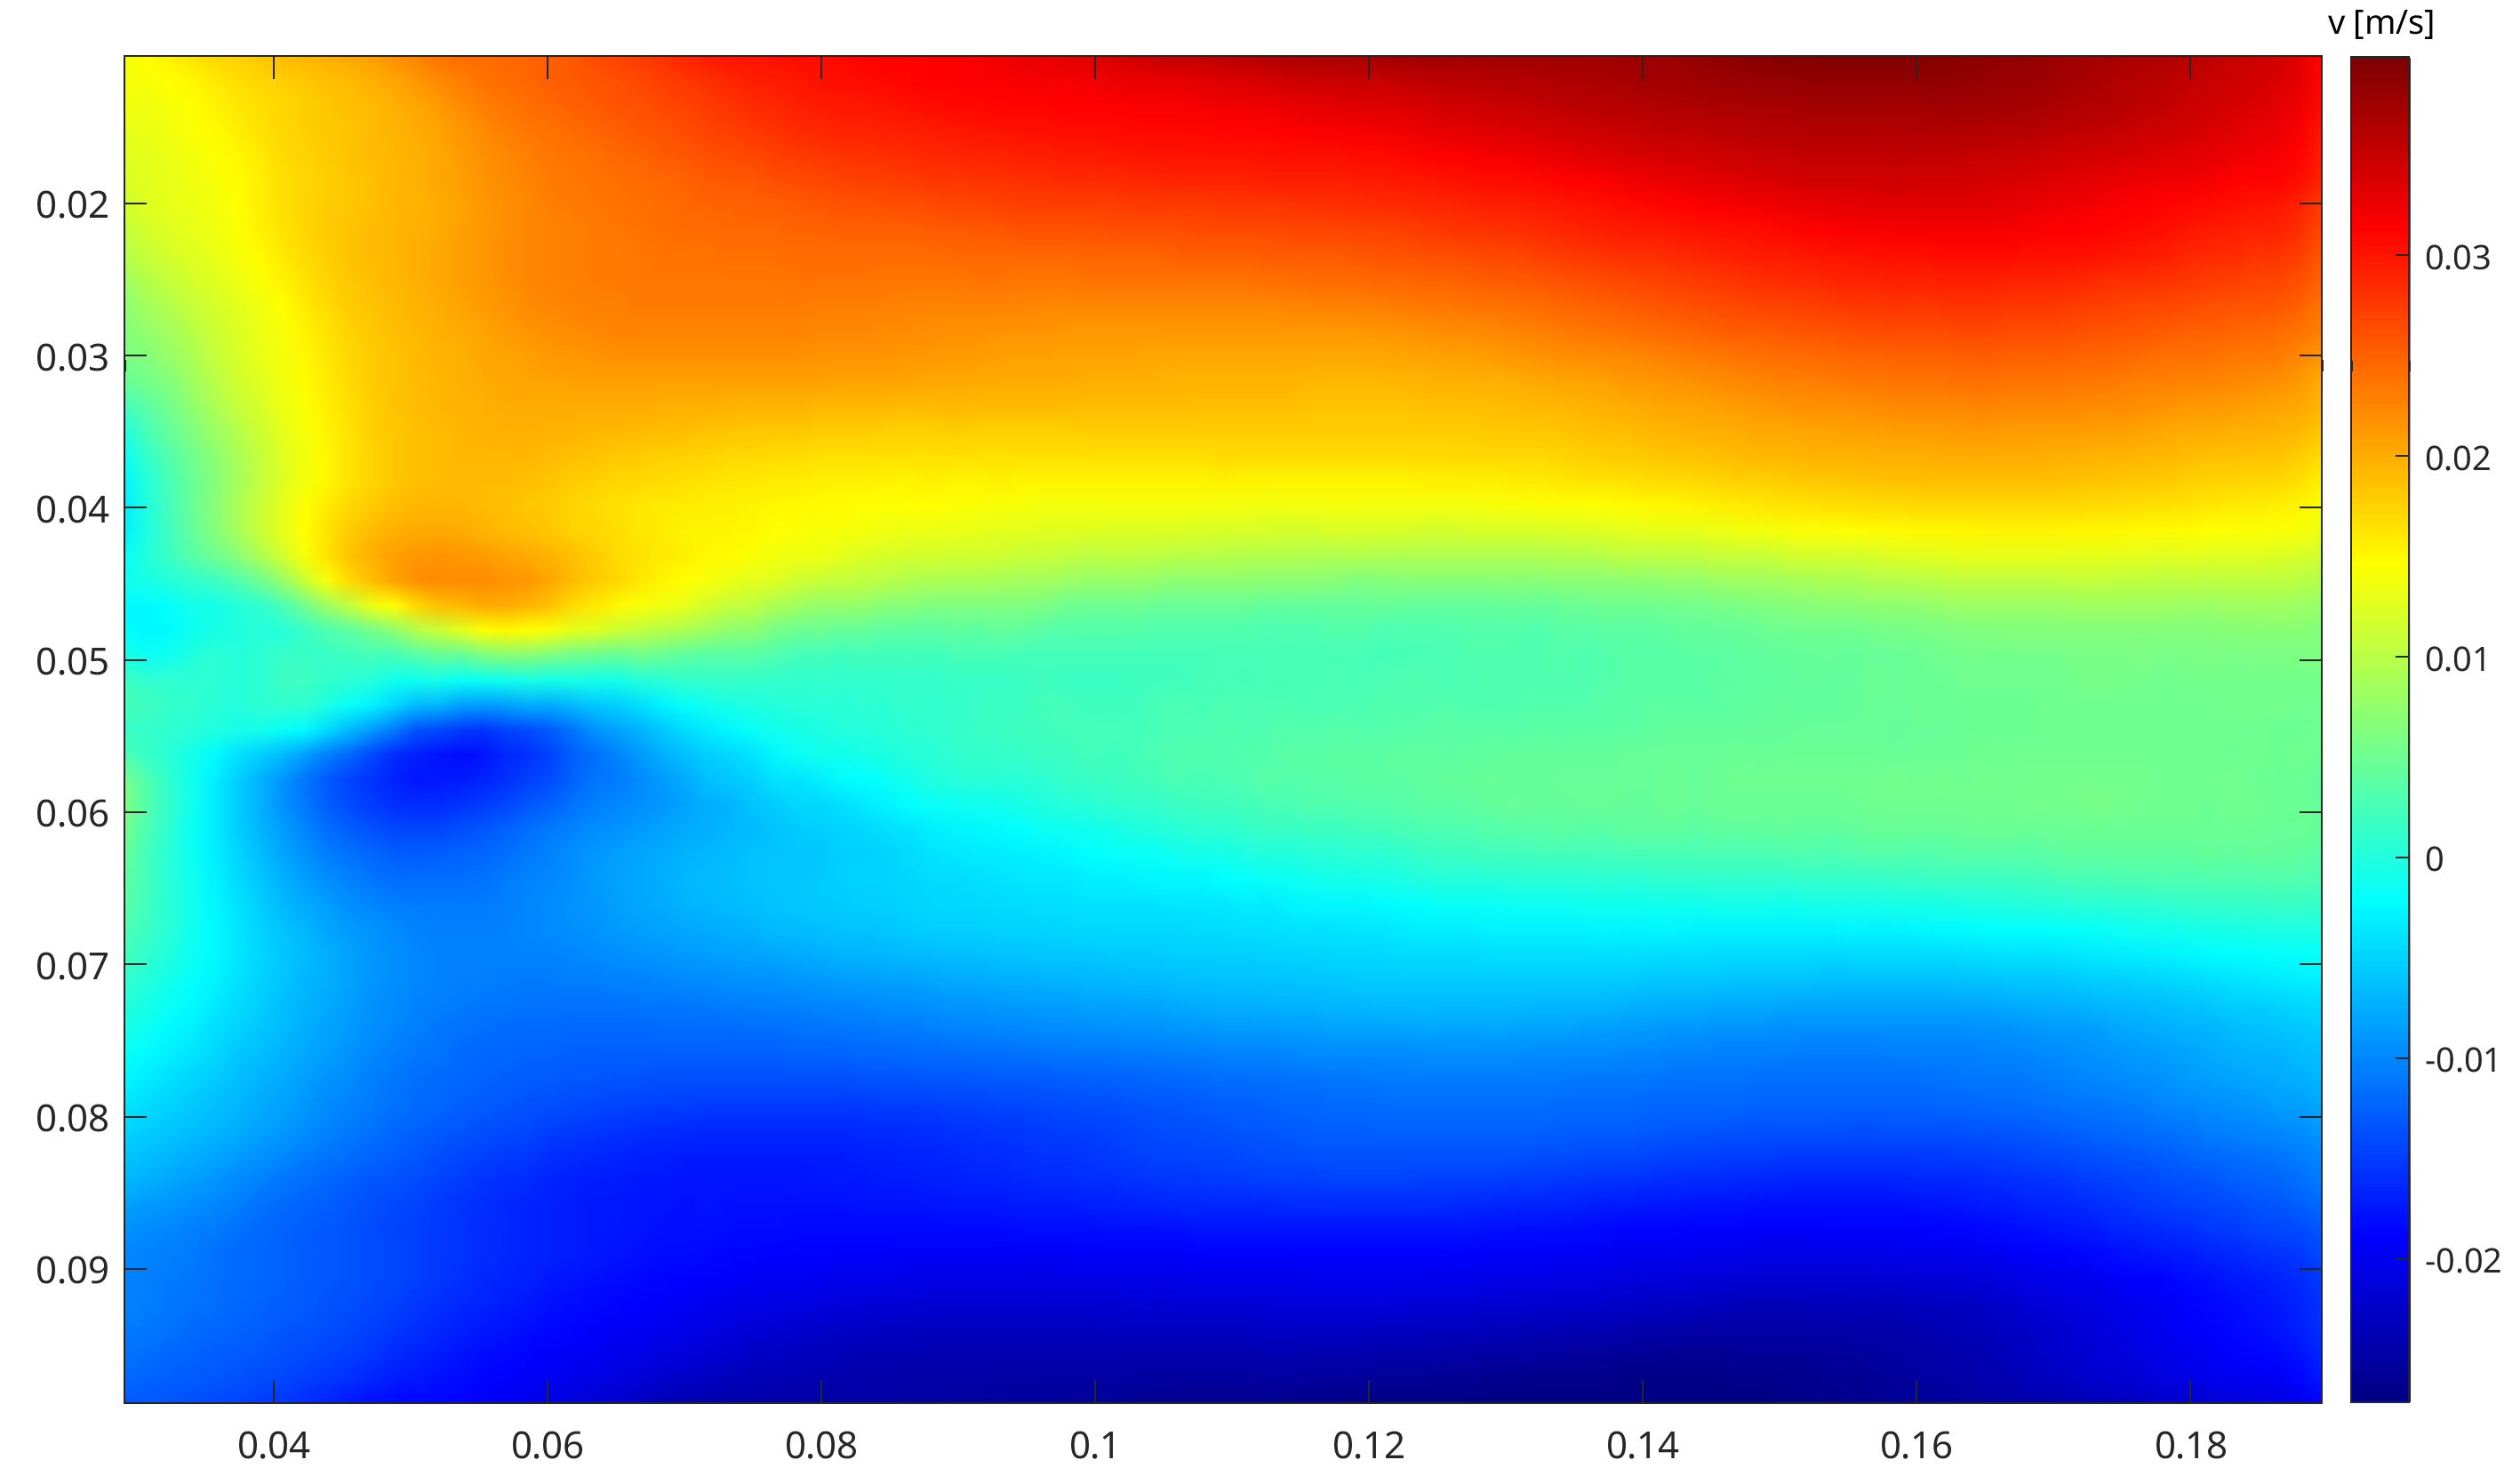
\includegraphics[width=.8\textwidth]{images/11/vmean.png}
    \caption{Componente trasversale della velocità media $v$ (cilindro 2022)}
\end{figure}

% DISCUTERE EVOLUZIONE DELLA VELOCITA' IN UN PUNTO FISSO (CIL 22, PLA 22)
\noindent Per studiare il vortex shedding si può tracciare un diagramma della velocità in un punto fisso nello spazio, in corrispondenza dei vortici che si generano. Si ottengono quindi i seguenti risultati:
\begin{figure}[H]
    \centering
    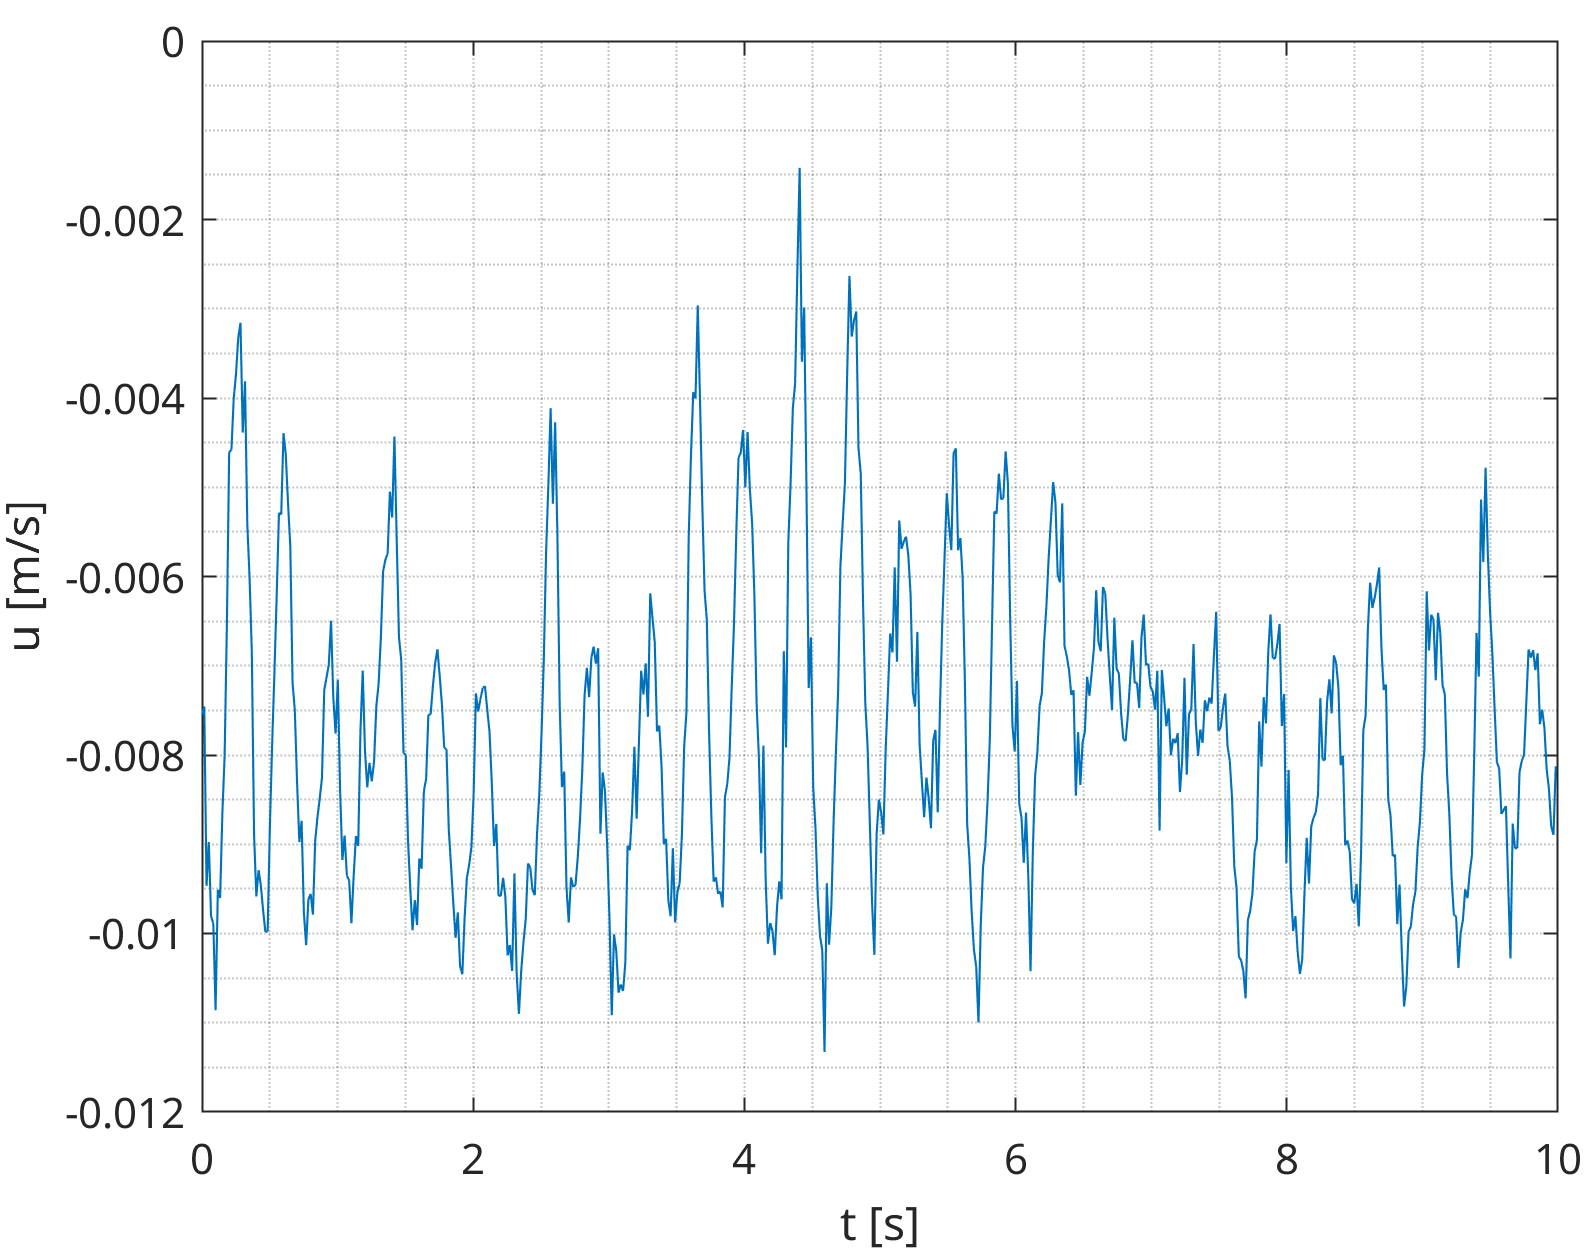
\includegraphics[width=.46\textwidth]{images/11/timeseries22.png}
    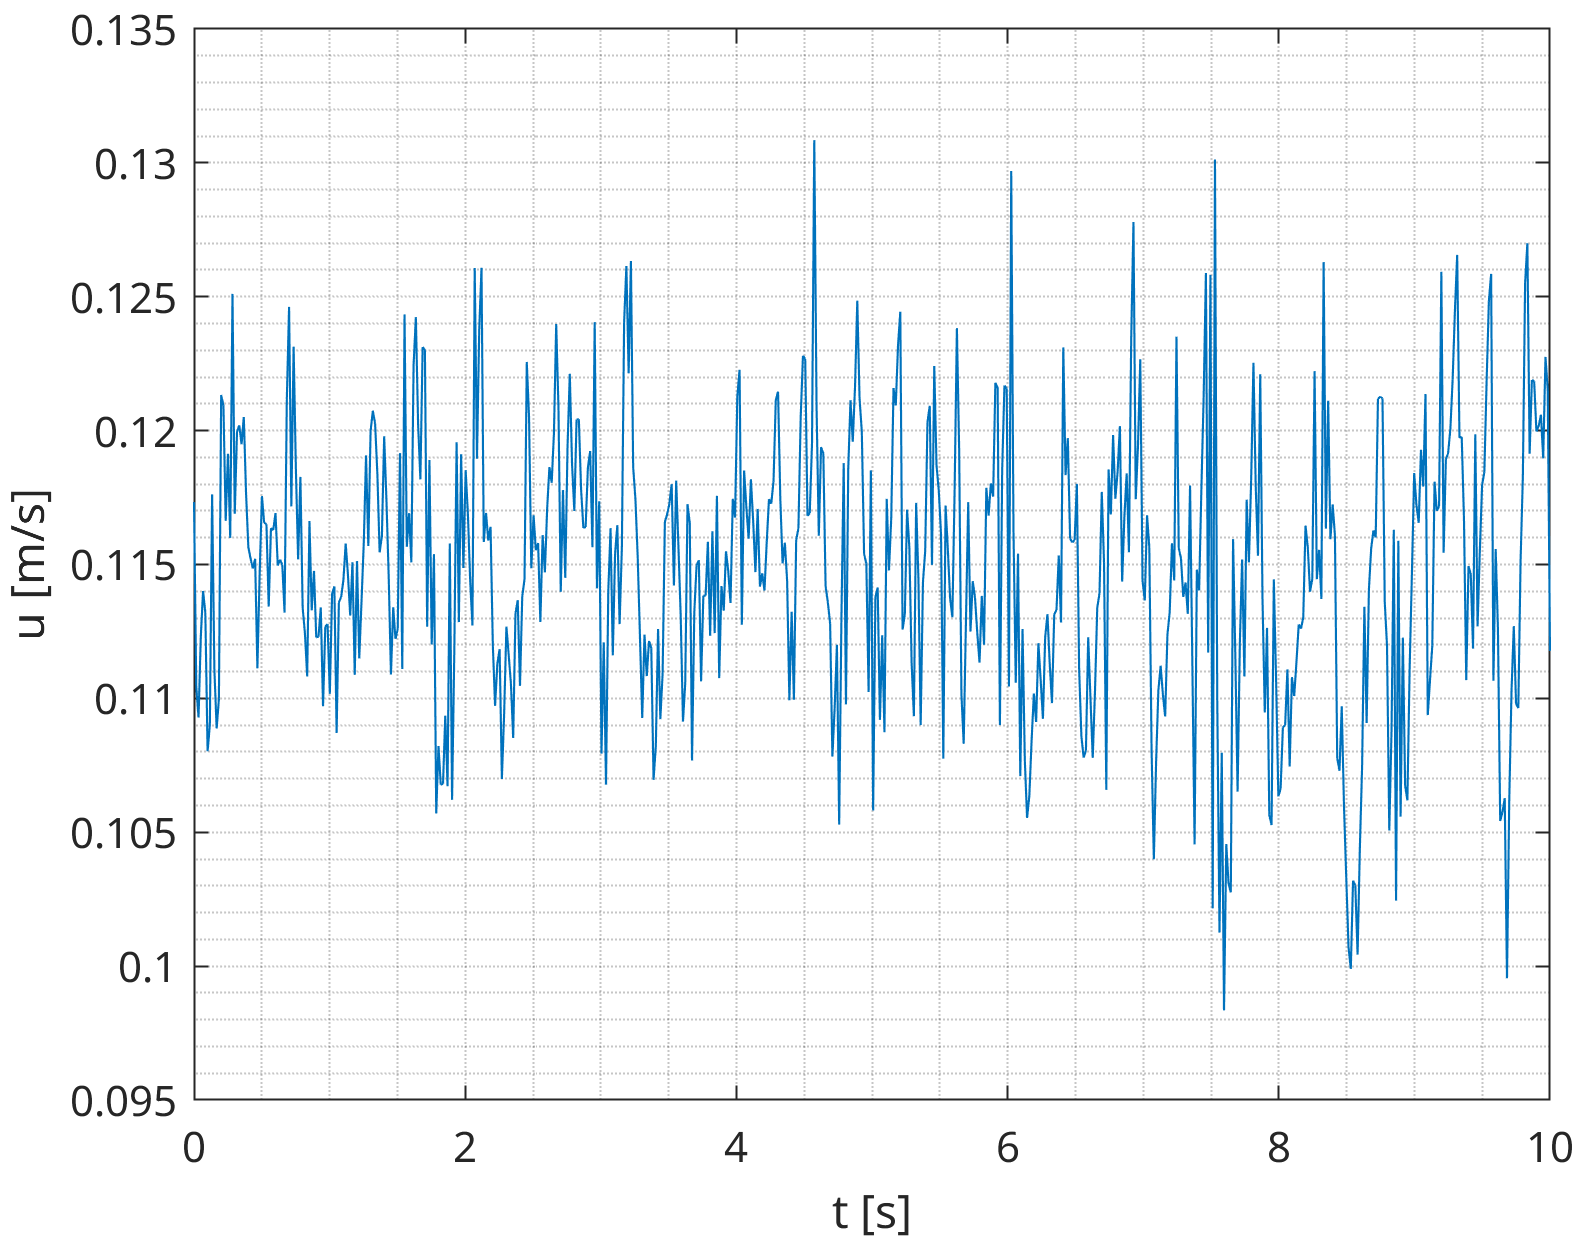
\includegraphics[width=.46\textwidth]{images/11/timeseries23.png}
    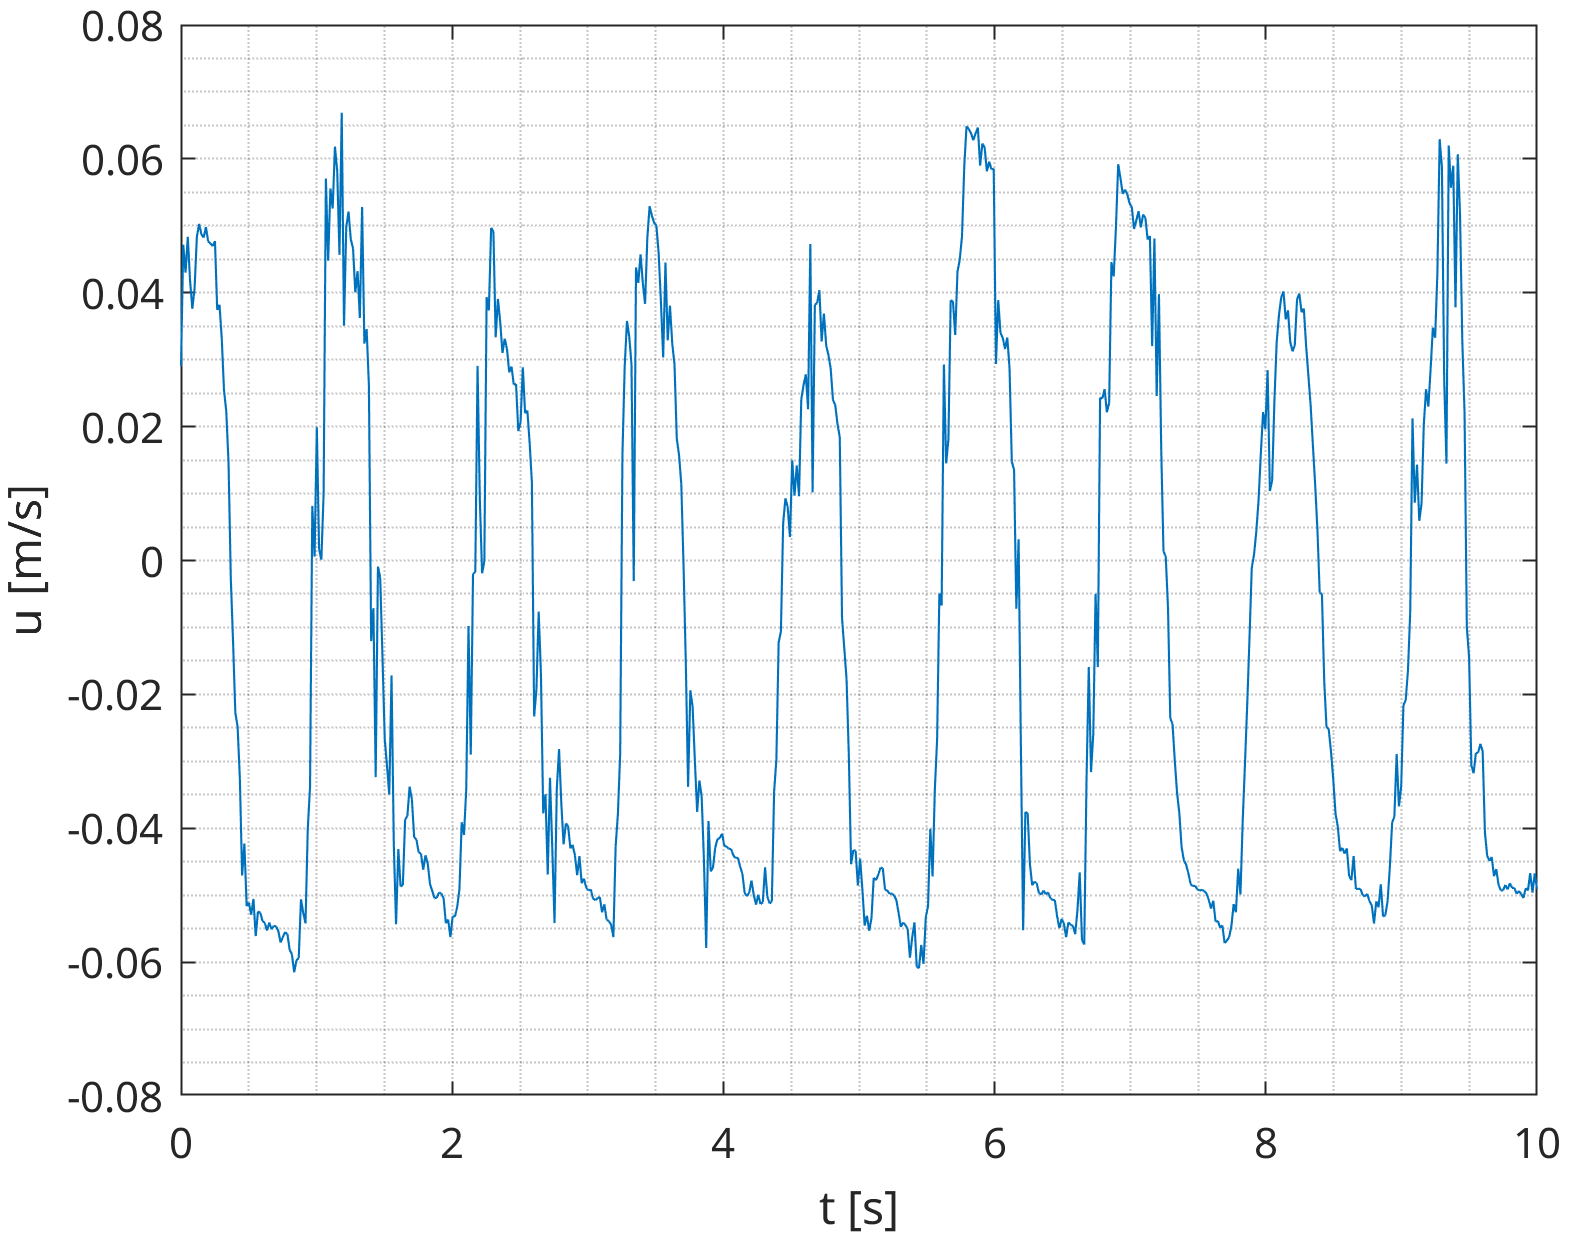
\includegraphics[width=.46\textwidth]{images/11/timeseries220.png}
    \caption{Velocità in un punto (cilindro 2022, cilindro 2023, placca 2022)}
\end{figure}

\noindent Dai diagrammi nel dominio del tempo si evince la presenza di una frequenza dominante, che caratterizza lo sfilamento vorticoso. Una rappresentazione più efficace può essere fatta sfruttando lo spettro di potenza.\\\\
Questa volta, però, il metodo di Welch non è una soluzione efficiente, in quanto il numero di frame acquisiti (600) è troppo basso per ottenere una stima accurata dello spettro di potenza utilizzando questo approccio. La frequenza di campionamento delle immagini (pari a $f_{samp}=60$ Hz) comporta, secondo il teorema di Nyquist, una massima frequenza rilevabile di 30 Hz. Tuttavia, dato che il segnale non presenta rumore significativo, è più efficiente utilizzare direttamente la FFT (Fast Fourier Transform):
\begin{equation*}
    \hat u(f) = \Delta t_{samp} \sum_{i=1}^{N_{frames}} u_i e^{-j2\pi f_i \Delta t_{samp}}
\end{equation*}
La FFT fornisce una rappresentazione spettrale accurata senza la necessità di segmentazione e sovrapposizione dei dati come nel metodo di Welch, risultando in un'analisi più semplice e diretta delle frequenze presenti.\\\\
Applicando la FFT ai segnali, si ottiene:
\begin{figure}[H]
    \centering
    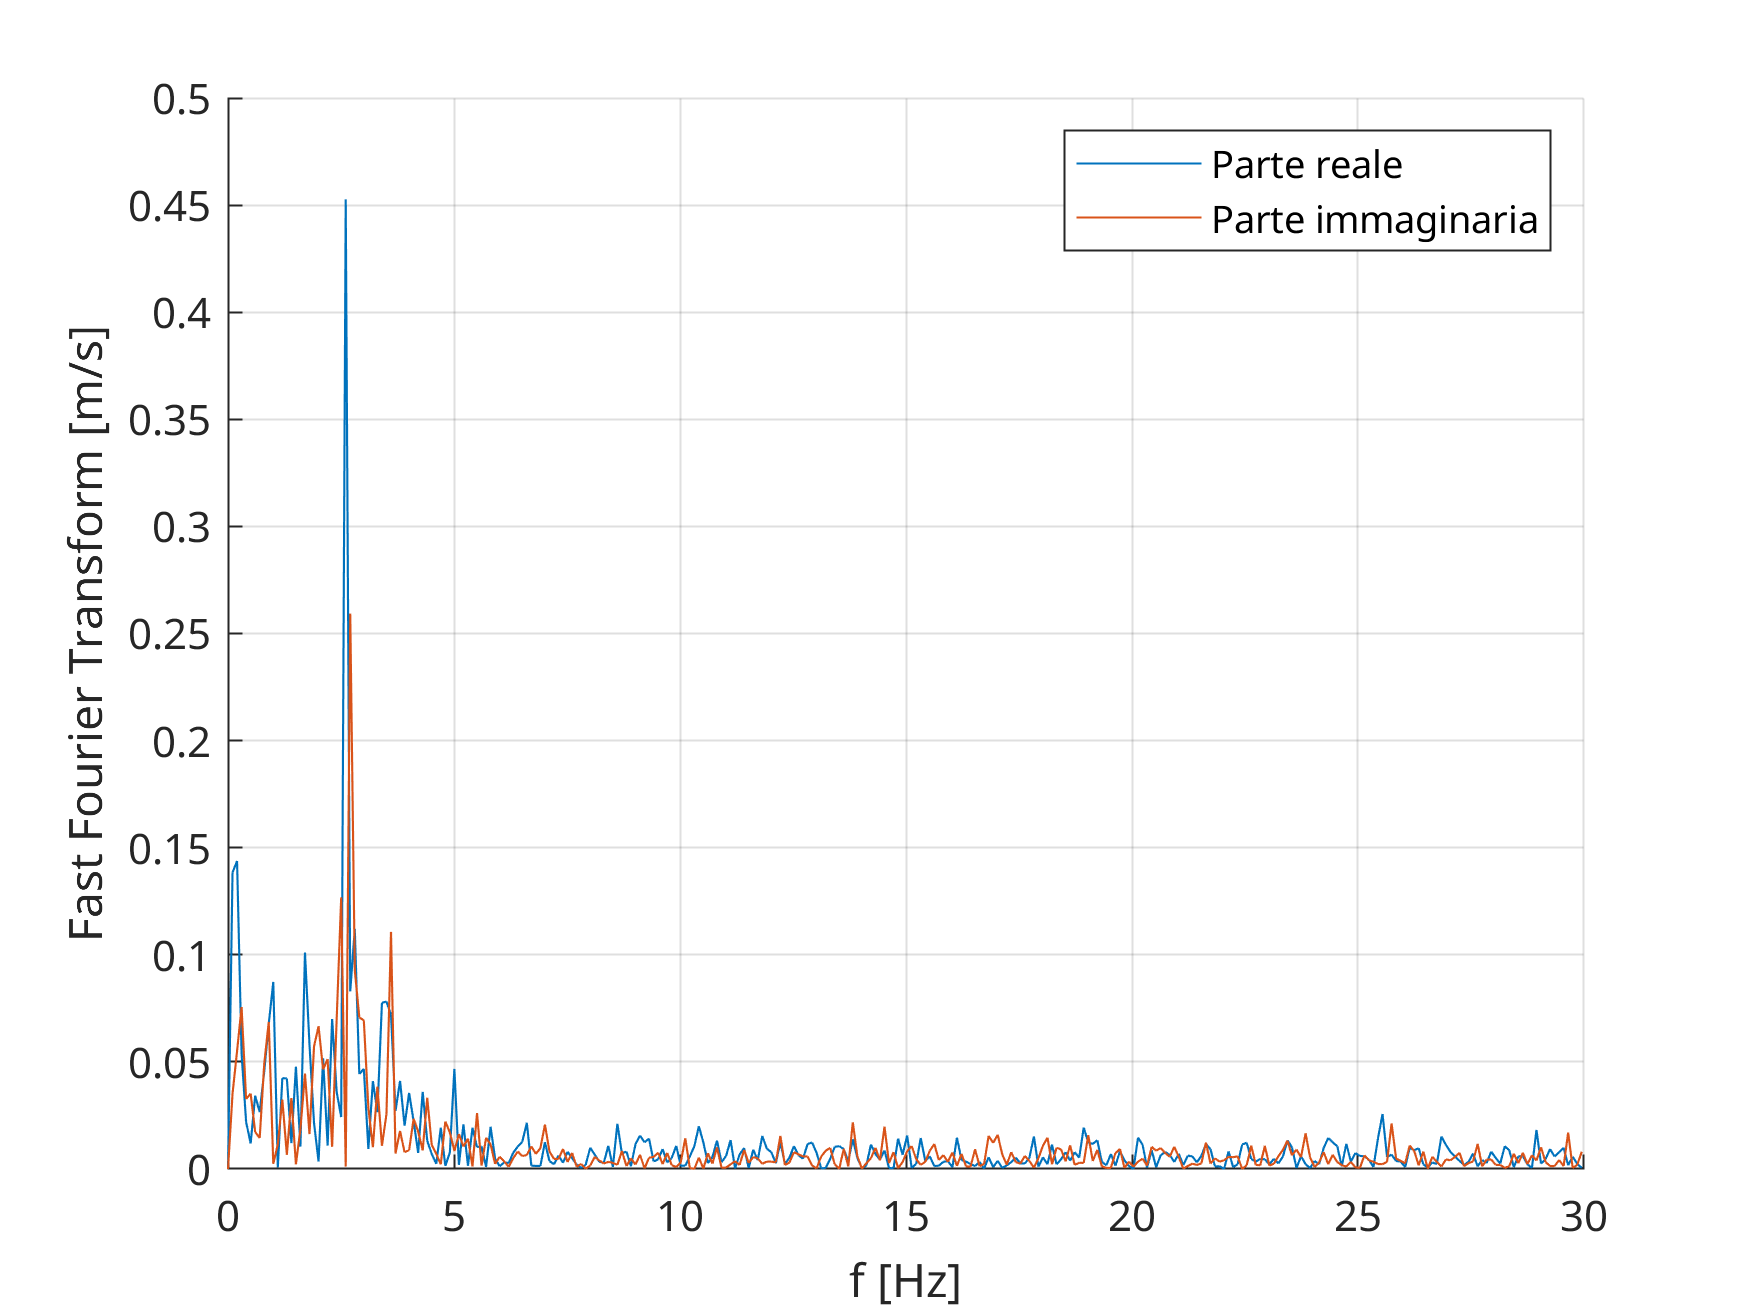
\includegraphics[width=.49\textwidth]{images/11/FFT22.png}
    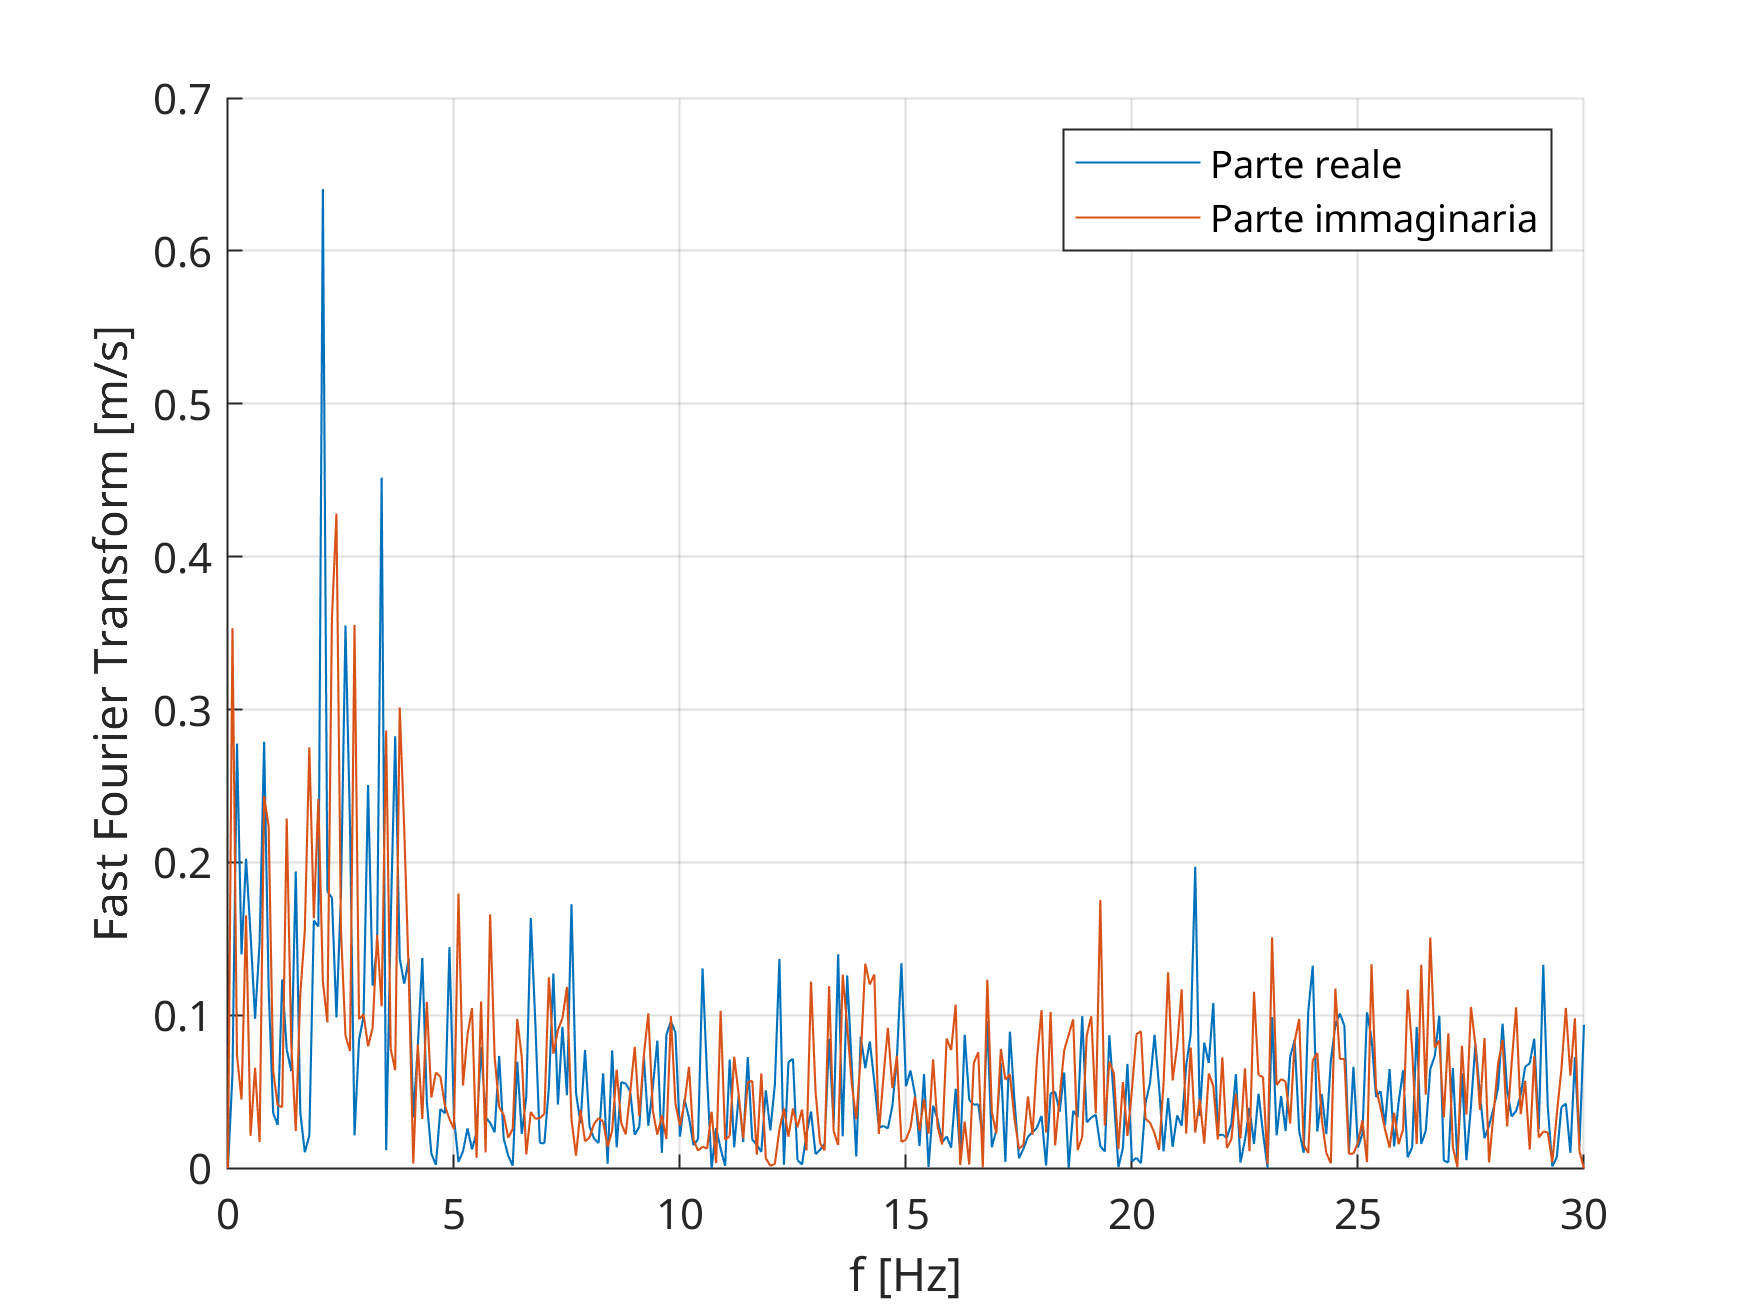
\includegraphics[width=.49\textwidth]{images/11/FFT23.png}
    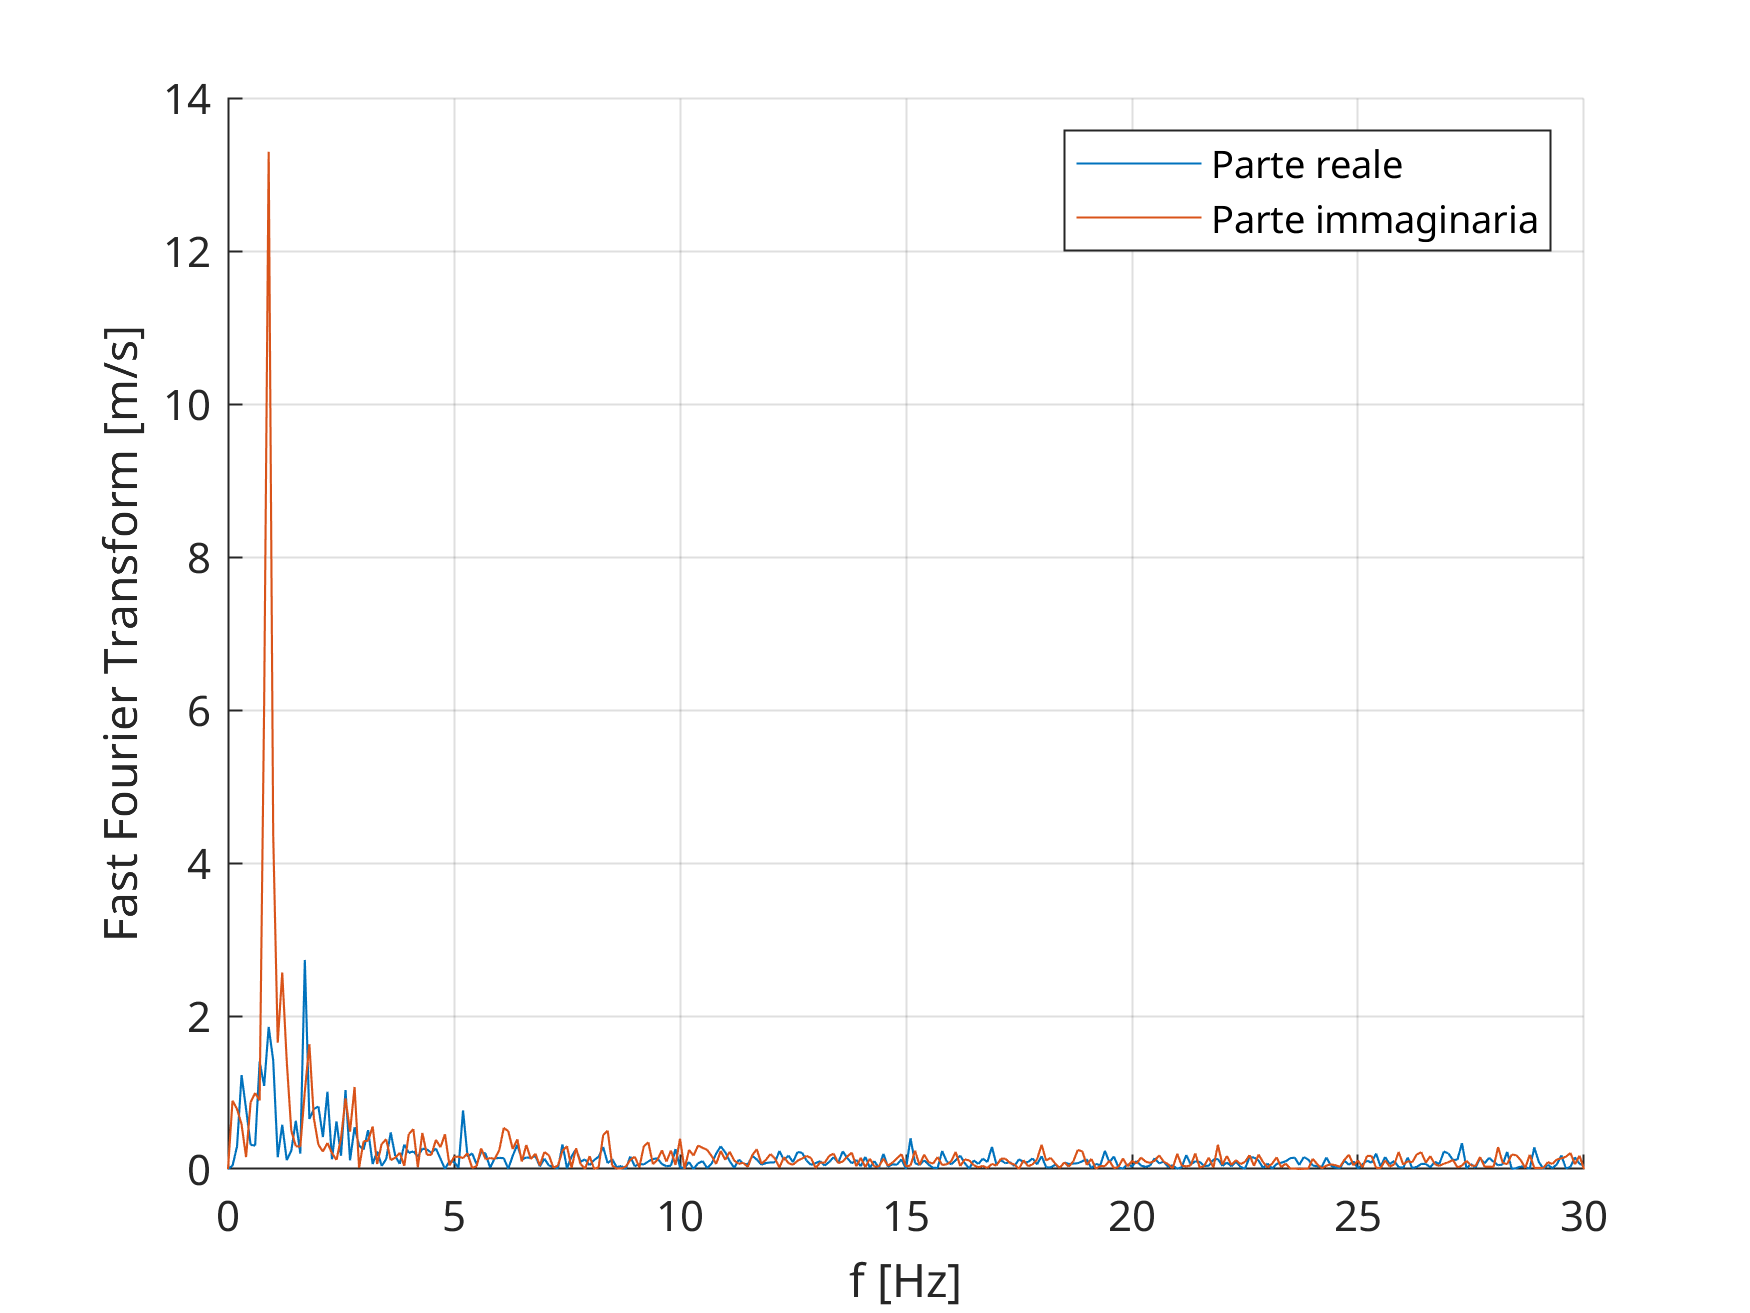
\includegraphics[width=.49\textwidth]{images/11/FFT220.png}
    \caption{Trasformata di Fourier (cilindro 2022, cilindro 2023, placca 2022)}
\end{figure}

\noindent Per ricavare lo spettro di potenza dai risultati della FFT, si calcola il modulo al quadrato e si normalizza rispetto al numero di fotogrammi $N_{frames}$:
\begin{equation*}
    P(f) = \left| \frac{\hat u(f)}{N_{frames}} \right|^2
\end{equation*}
\begin{figure}[H]
    \centering
    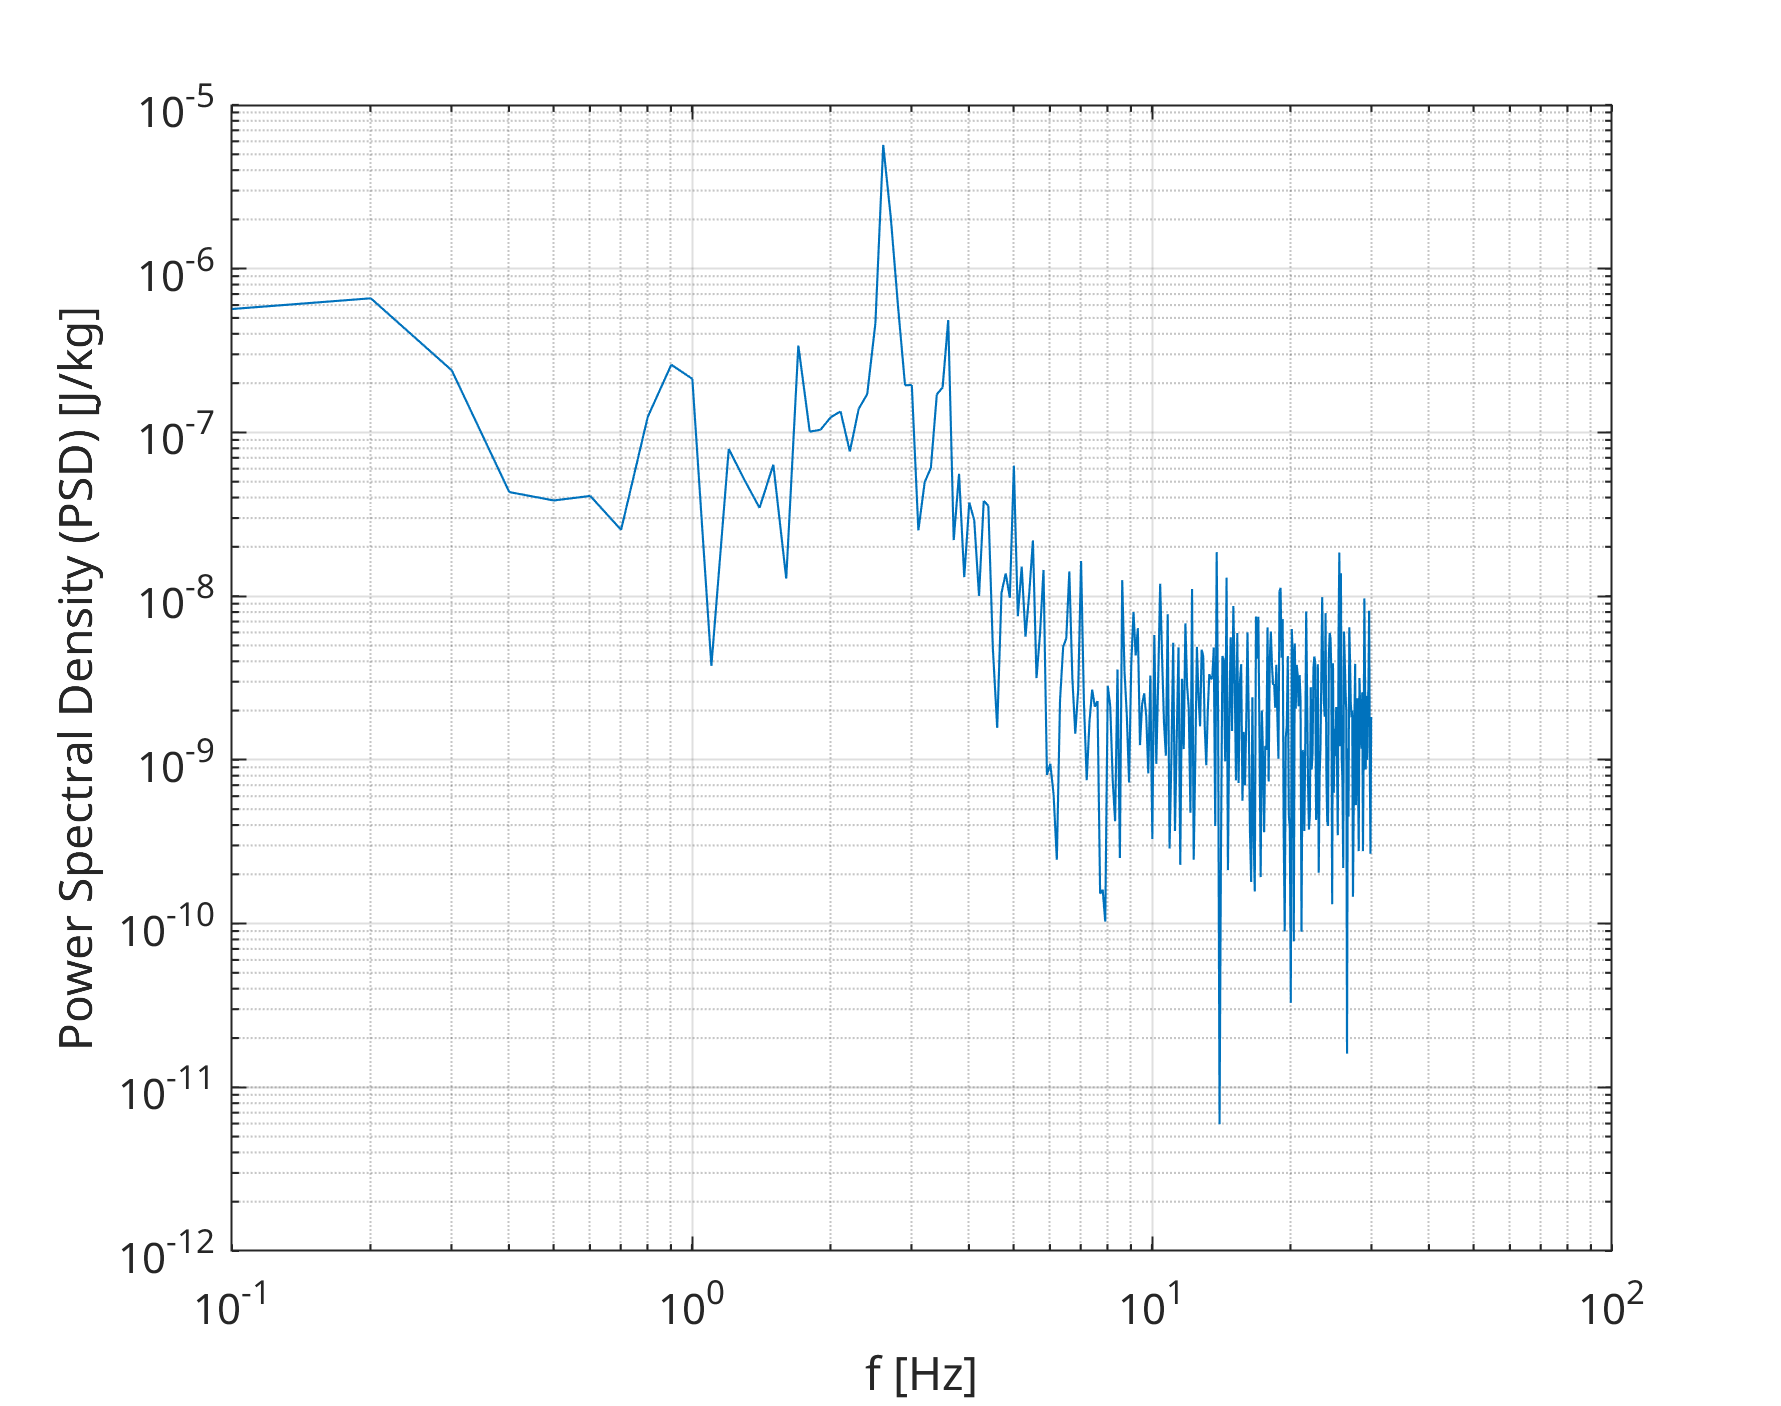
\includegraphics[width=.49\textwidth]{images/11/PSD22.png}
    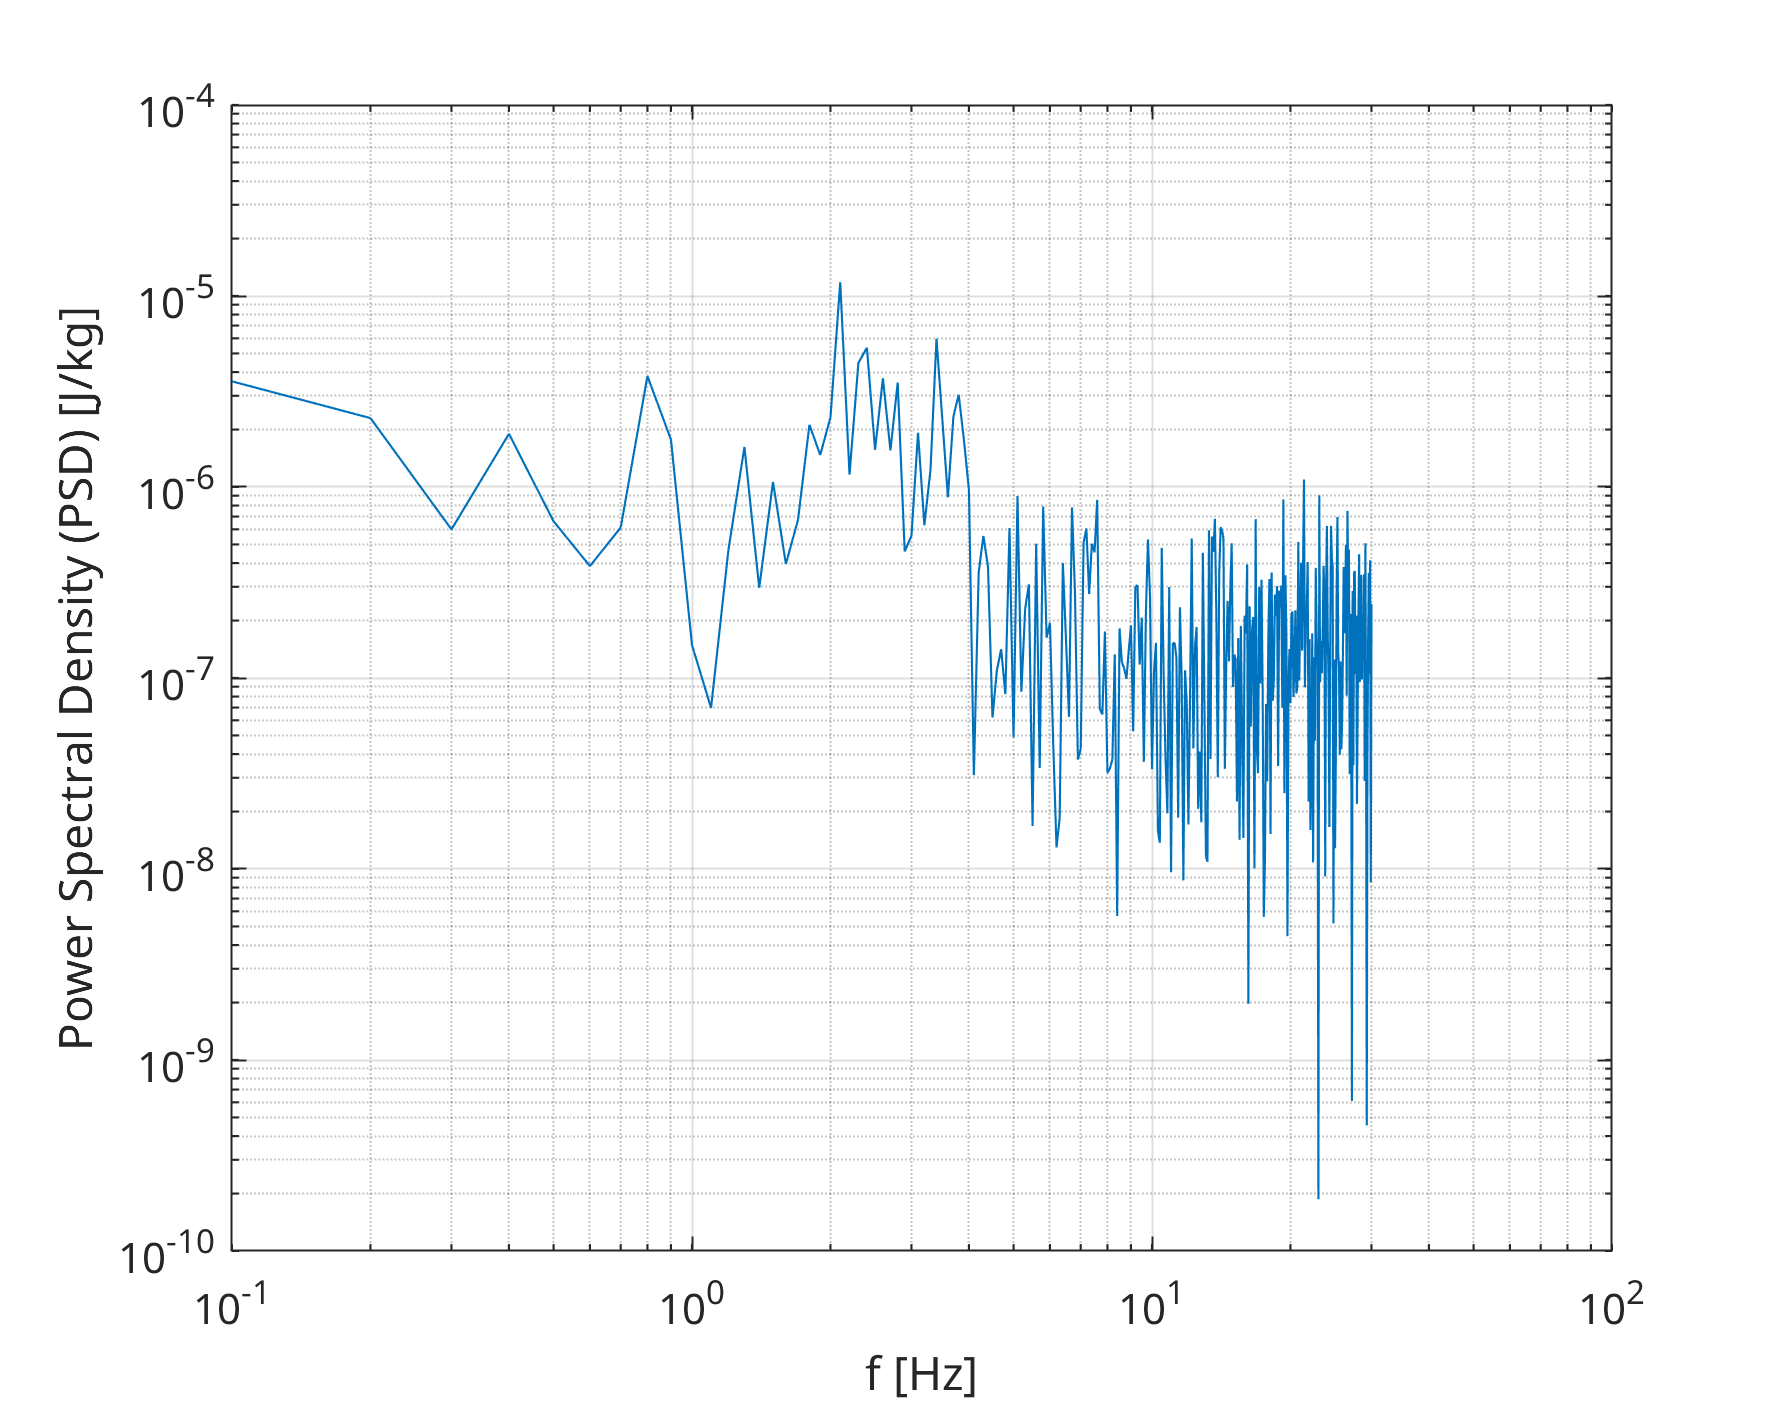
\includegraphics[width=.49\textwidth]{images/11/PSD23.png}
    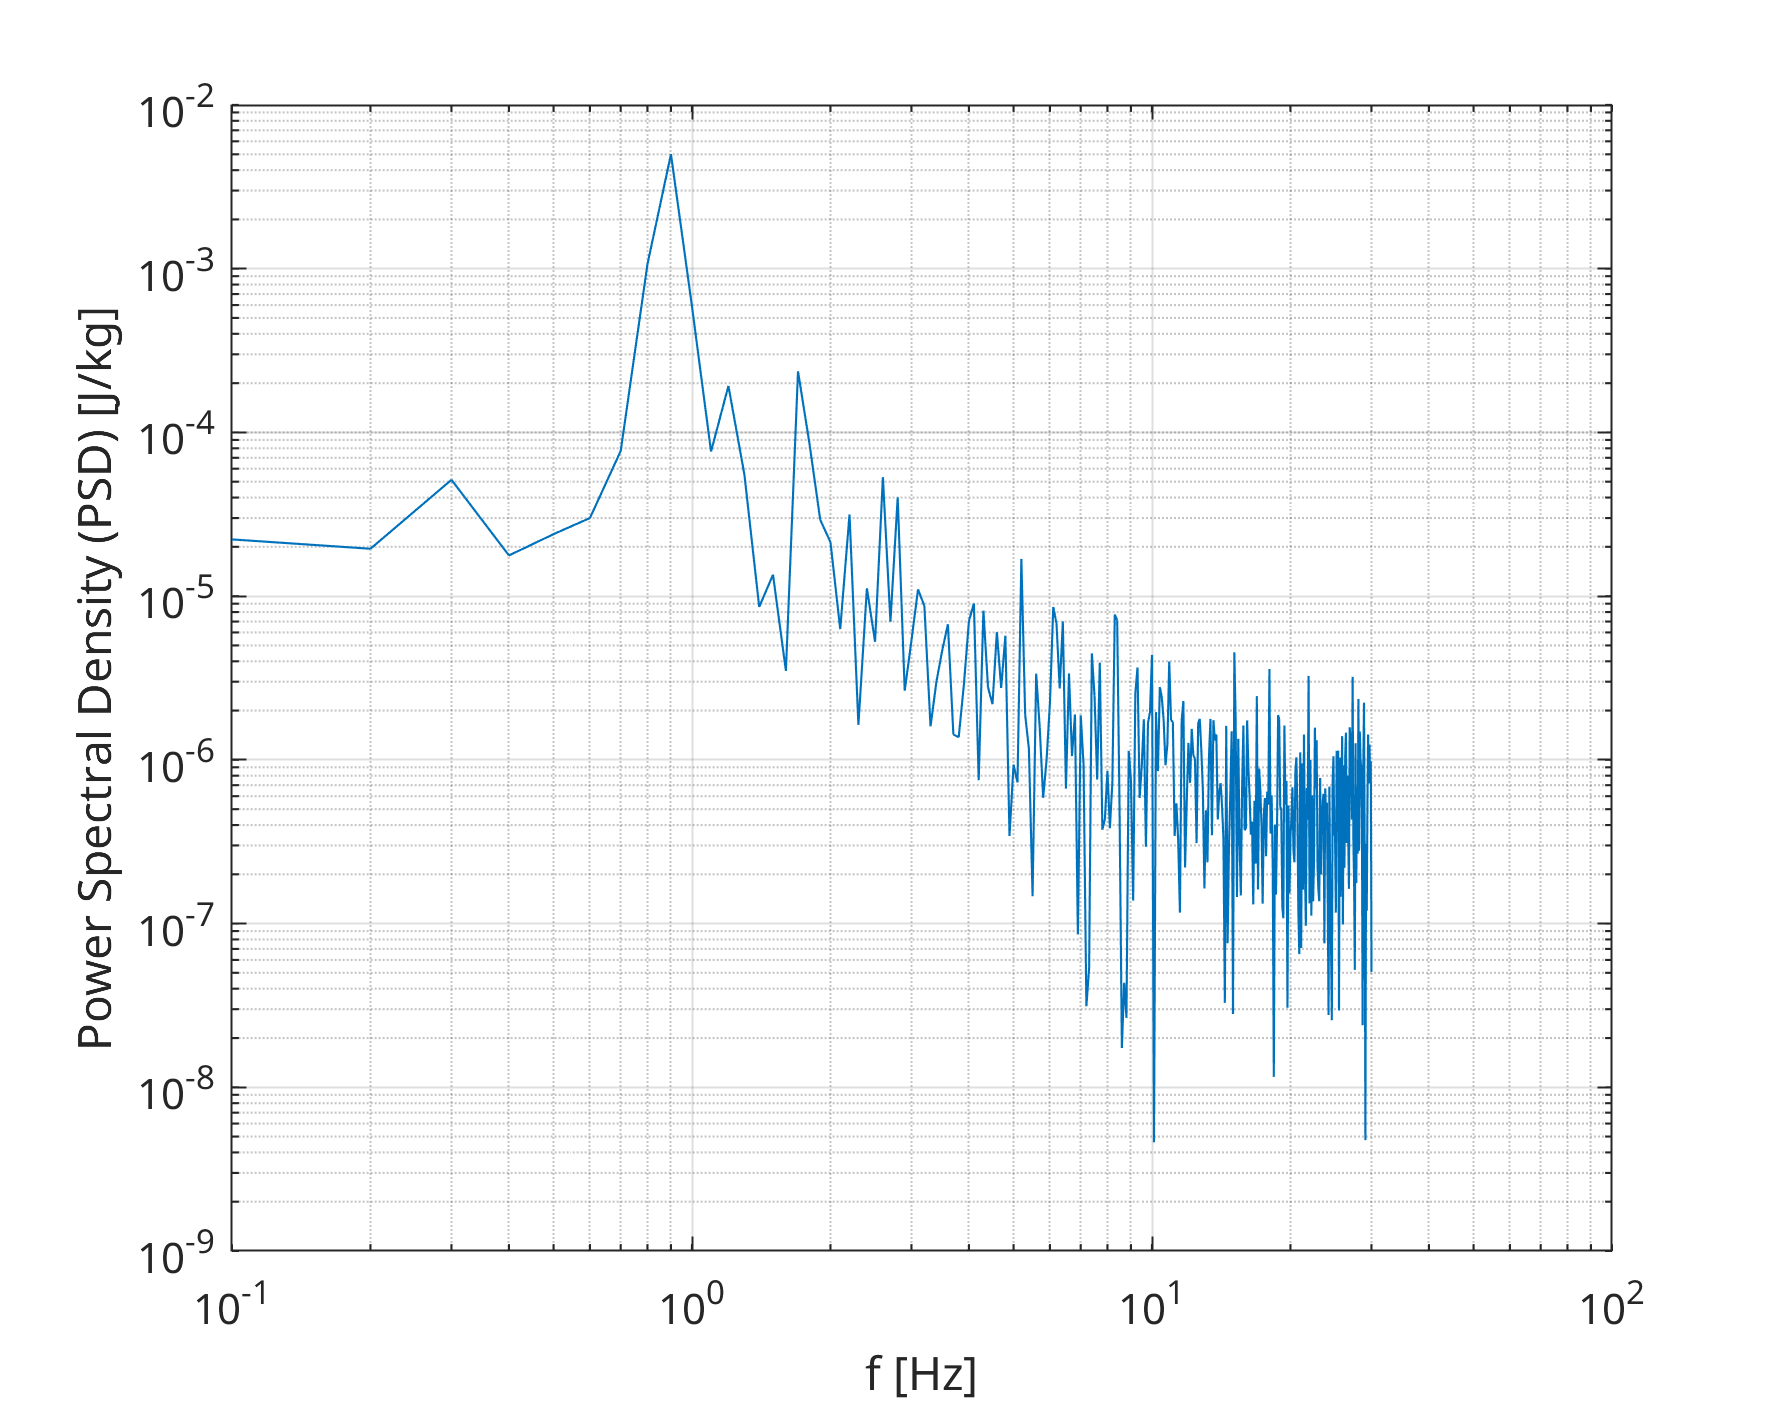
\includegraphics[width=.55\textwidth]{images/11/PSD220.png}
    \caption{Spettro di potenza (cilindro 2022, cilindro 2023, placca 2022)}
\end{figure}

\noindent Dallo spettro di potenza si ricava la frequenza di shedding $f_s$, inoltre, si può stimare la velocità a monte del flusso $U_\infty$ da un punto non influenzato dai vortici. Si ottiene:
\begin{table}[H]
    \centering
    \begin{tabular}{|c|c|c|}
    \hline
    Caso          & $f_s$   & $U_\infty$ \\ \hline
    Cilindro 2022 & 2.60 Hz & 0.121 m/s  \\ \hline
    Cilindro 2023 & 2.10 Hz & 0.114 m/s  \\ \hline
    Placca 2022   & 0.90 Hz & 0.090 m/s  \\ \hline
    \end{tabular}
\end{table}

\noindent Dal valore di velocità a monte si ricava il numero di Reynolds:
\begin{equation*}
    Re = \frac{U_\infty D}{\nu_{H_2O} }
\end{equation*}
dove $D$ rappresenta una lunghezza caratteristica del corpo esaminato (diametro per il cilindro o lunghezza per la placca piana), mentre $\nu_{H_2O}$ è la viscosità cinematica dell'acqua ($\nu_{H_2O}\approx 9.31\cdot10^{-7}$ m$^2$/s). Con la frequenza di shedding $f_s$ si ricava invece il numero di Strouhal:
\begin{equation*}
    St = \frac{f_s D}{U_\infty}
\end{equation*}
Si ottengono i seguenti risultati:
\begin{table}[H]
    \centering
    \begin{tabular}{|c|c|c|c|c|}
    \hline
    Caso          & $f_s$   & $U_\infty$ & Reynolds & Strouhal \\ \hline
    Cilindro 2022 & 2.60 Hz & 0.121 m/s  & 1296     & 0.215    \\ \hline
    Cilindro 2023 & 2.10 Hz & 0.114 m/s  & 1225     & 0.185    \\ \hline
    Placca 2022   & 0.90 Hz & 0.090 m/s  & 2331     & 0.239    \\ \hline
    \end{tabular}
\end{table}

\noindent Nel caso del cilindro, si possono confrontare i risultati ottenuti con il diagramma Reynolds-Strouhal dell'attività precedente:
\begin{figure}[H]
    \centering
    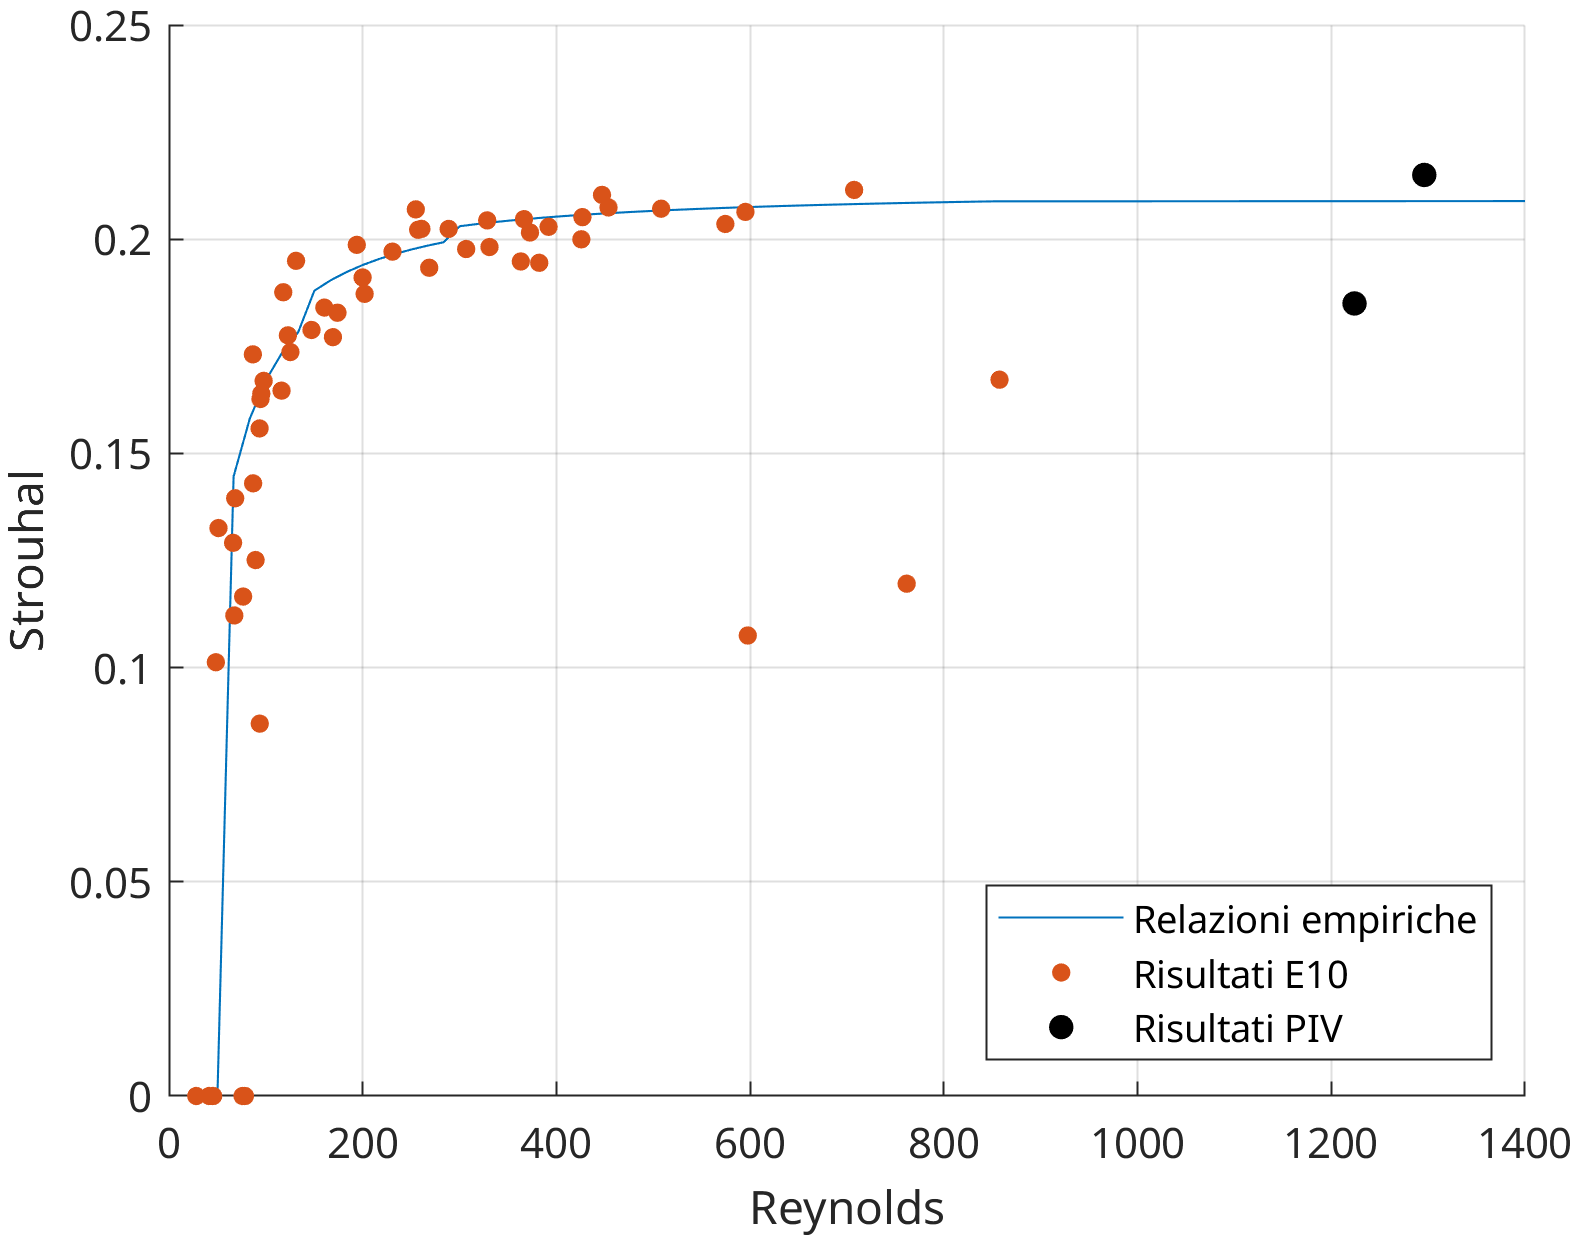
\includegraphics[width=.75\textwidth]{images/11/Re-St.png}
    \caption{Diagramma Reynolds-Strouhal}
\end{figure}

\noindent Il flusso che si sviluppa non risulta essere quello canonico 2D per via della sua dimensione finita che appoggia sulla parete inferiore della camera di prova. Inoltre, il piano di misura è a un diametro di distanza dal fondo, dove si sviluppa il vortice a ferro di cavallo (horseshoe vortex) e sono presenti effetti tridimensionali dovuti all'induzione del vortice. Per questi motivi i casi da studiare differiscono dai flussi canonici bidimensionali, pertanto, l'andamento Reynolds-Strouhal si discosta leggermente da quello studiato per il cilindro 2D utilizzando l'anemometria a filo caldo.
\newpage
\noindent Si procede al calcolo delle fluttuazioni di velocità sottraendo in ogni punto la velocità media temporale:
\begin{equation*}
    u^\prime(t) = u(t) - \overline u \qquad v^\prime(t) = v(t) - \overline v  
\end{equation*}
Dalle fluttuazioni si può ricavare la varianza:
\begin{equation*}
    \text{var}(\vec V) = \overline{{V^\prime}^2} = \frac 1{N_{frames}} \sum ({u^\prime}^2 + {v^\prime}^2)
\end{equation*}
Per il teorema di Parisval, la varianza risulta pari a:
\begin{equation*}
    \overline{{V^\prime}^2} = \int_0^{\frac{f_{samp}}2} P(f) df
\end{equation*}
Dal campo di fluttuazioni di velocità si possono inoltre ricavare gli sforzi di Reynolds:
\begin{equation*}
    \tau_{Re} = -\rho \overline{u^\prime v^\prime}
\end{equation*}
Si ottiene quindi il seguente diagramma:
\begin{figure}[H]
    \centering
    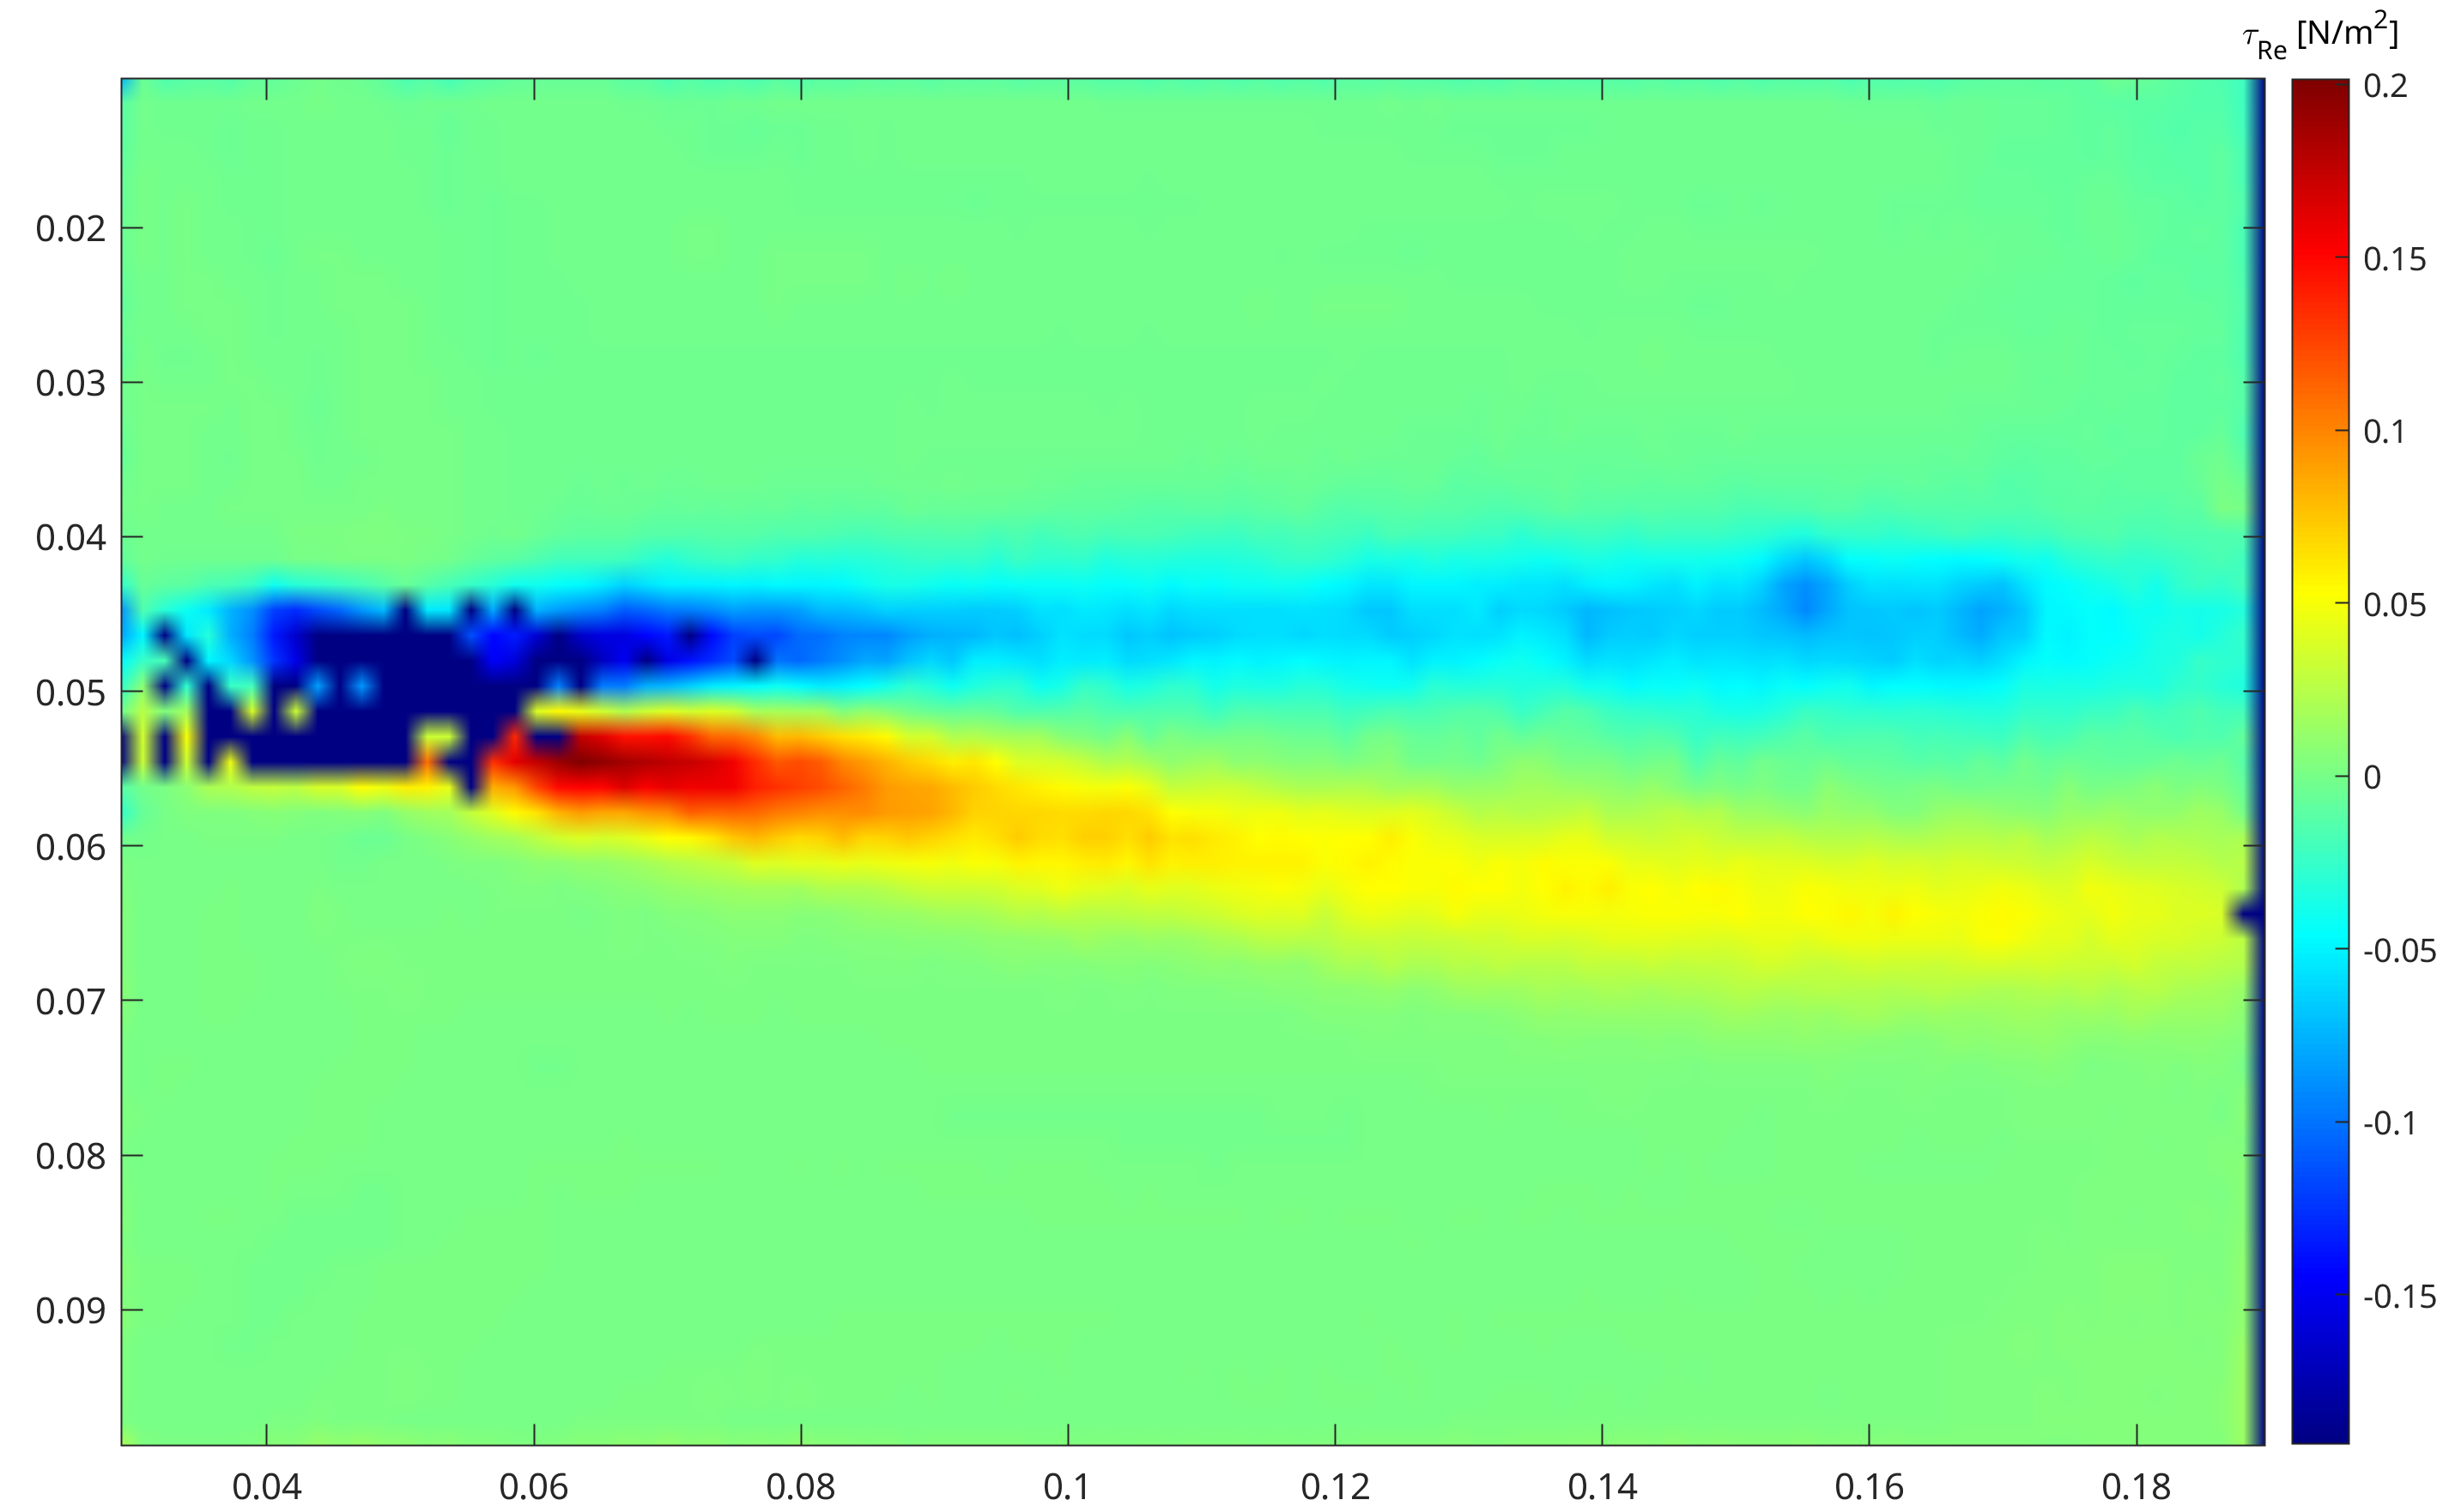
\includegraphics[width=\textwidth]{images/11/tauRe.png}
    \caption{Sforzi di Reynolds (cilindro 2022)}
\end{figure}